\documentclass[lettersize,journal]{IEEEtran}
\usepackage{amsmath,amsfonts}
\usepackage{algorithmic}
\usepackage{algorithm}
\usepackage{array}
\usepackage[caption=false,font=normalsize,labelfont=sf,textfont=sf]{subfig}
\usepackage{textcomp}
\usepackage{stfloats}
\usepackage{url}
\usepackage{verbatim}
\usepackage{graphicx}
\usepackage{cite}
\hyphenation{op-tical net-works semi-conduc-tor IEEE-Xplore}
% updated with editorial comments 8/9/2021

\newcommand{\new}[1]{\textcolor{blue}{#1}}
\newcommand{\EE}{\text{E}}
\newcommand{\HD}{\text{HD}}

%\usepackage{lineno,hyperref}
%hyperref does not compile with JAIR
%\modulolinenumbers[5]

%\usepackage{natbib}

\usepackage{epstopdf}
\usepackage{lineno}
\usepackage{amsthm}

\usepackage{multirow}

\usepackage{booktabs} % For formal tables
\usepackage{csquotes}

\usepackage{amsmath}
\usepackage{amssymb}
\usepackage{setspace}
\usepackage{graphicx} 
\hyphenation{methods}

\usepackage{csquotes}
\usepackage{mathtools}
\usepackage{algorithm}
\usepackage{algorithmic}
\usepackage{caption}
\usepackage{thmtools,thm-restate}
\usepackage{url}
%\usepackage{subcaption}

\usepackage{xcolor}


\newcommand{\prob}[1]{\Pr\left(#1\right)}
%\newcommand{\oneoneiahype}{$(1+1)~\text{IA}$}
\newcommand{\oneonerlsone}{$(1+1)~\text{RLS}$}
\newcommand{\oneoneIA}{$(1+1)$~IA}
\newcommand{\oneoneOPTIA}{$(1+1)$~Opt-IA}
\newcommand{\jumpcliff}{\textsc{JumpCliff}~}
\newcommand{\cliff}{\textsc{Cliff}$_d$}
\newcommand{\onemax}{\textsc{OneMax}}
\newcommand{\leadingones}{\textsc{LeadingOnes}}
\newcommand{\twomax}{\textsc{TwoMax}}
\newcommand{\trunmax}{\textsc{TruncatedTwoMax}}
\newcommand{\jump}{\textsc{Jump}$_k$}
\newcommand{\linHD}{M$_{\text{linHD}}$}
\newcommand{\expoF}{M$_{\text{expoF(x)}}$}
\newcommand{\expoHD}{M$_{\text{expoHD}}$}
\newcommand\T{\rule{0pt}{2.6ex}}      
\newcommand\B{\rule[-1.2ex]{0pt}{0pt}}

%\newcommand{\invB}{$(1+1)~\text{IA}_{inv\beta}~$}
%\newcommand{\hypero}{invHype}
\newcommand{\fastea}{$(1+1)$Fast EA}
\newcommand{\blin}{$\beta_{\text{linHD}}$}
\newcommand{\bexpo}{$\beta_{\text{expoHD}}$}
\newcommand{\Sbexpo}{Symmetric $\beta_{\text{expoHD}}$}

\newcommand{\IPHfcm}{IPH}
%\newcommand{\IPHbeta}{IPH$_{\beta}$}


\newtheorem{theorem}{Theorem}
\newtheorem{corollary}{Corollary}
\newtheorem{property}{Property}
\newtheorem{lemma}{Lemma}
\newtheorem{definition}{Definition}

%\newcommand*{\oneoneea}{($\mu$+1)~GA\xspace}


\hyphenation{a-na-ly-sis}
\hyphenation{Leading-Ones}
\hyphenation{ge-ne-ration}
\hyphenation{ge-ne-rations}
\hyphenation{cha-racte-ris-tics}
\begin{document}

\title{Effective Inversely Proportional Hypermutations for Unimodal and Multimodal Optimisation}

\author{IEEE Publication Technology,~\IEEEmembership{Staff,~IEEE,}	
        % <-this % stops a space
        
}
%\author{IEEE Publication Technology,~\IEEEmembership{Staff,~IEEE,}	
%	% <-this % stops a space
	\author{Anonymous authors	
	% <-this % stops a space

}

% The paper headers
\markboth{Journal of \LaTeX\ Class Files,~Vol.~14, No.~8, August~2021}%
{Shell \MakeLowercase{\textit{et al.}}: A Sample Article Using IEEEtran.cls for IEEE Journals}

%\IEEEpubid{0000--0000/00\$00.00~\copyright~2021 IEEE}
% Remember, if you use this you must call \IEEEpubidadjcol in the second
% column for its text to clear the IEEEpubid mark.

\maketitle

\begin{abstract}
Artificial Immune Systems (AIS) employing hypermutations with linear static mutation potential have recently been shown to be very effective at escaping local optima of combinatorial optimisation problems
at the expense of being slower during the exploitation phase compared to standard evolutionary algorithms.
In this paper, we prove that considerable speed-ups in the exploitation phase may be achieved 
with dynamic inversely proportional  hypermutations (IPH) with mutation potentials
and argue that the potential should decrease inversely to the distance to the optimum rather than to the difference in fitness as in the literature. Afterwards, we define a simple (1+1)~Opt-IA that uses IPH and ageing for realistic applications where optimal solutions are unknown. 
%
%with dynamic mutation potentials that are inversely proportional to the optimum (IPM)
%if inversely proportional mutation potentials (IPM) are used 
%instead of static ones
%We first prove that the desired behaviour is achieved for several benchmark functions if the optimum is known  
%and argue that the potential should decrease inversely to the distance to the optimum rather than with the difference in fitness. Afterwards, we define a simple (1+1)~Opt-IA artificial immune system, that uses IPM hypermutations and ageing, for realistic applications where optimal solutions are unknown. 
The aim of this AIS is to approximate the ideal behaviour of the IPH better and better as the search space is explored.
We prove that such desired behaviour and related speed-ups occur for unimodal functions as well as for well-studied bimodal benchmark functions %called \textsc{TwoMax}.
%Furthermore, we prove that the (1+1)~Opt-IA with IPM efficiently optimises a second multimodal function, \textsc{Cliff}, by escaping its local optima while Opt-IA with static mutation potential cannot, requiring exponential expected runtime in 
%the distance between the local and global optima.
which are hard to optimise for traditional evolutionary algorithms and for AIS using static mutation potentials.
\end{abstract}

\begin{IEEEkeywords}
Artificial immune systems, heavy-tailed mutations, inversely proportional hypermutations, theory, runtime analysis
\end{IEEEkeywords}

\section{Introduction}
Three recent hot topics in the theory of randomised search heuristics for optimisation in general and in artificial intelligence in particular have been the benefits of mutation operators with higher mutation rates than traditionally employed and recommended \cite{FQWGECCO18,FGQWPPSN18,CorusOlivetoYazdani2021TEVC,DoerrGECCO2017FastGA,CorusOlivetoTEVCsteadyGA2017,JumpTEVC2017,CorusOlivetoGecco2019,OlivetoSudholtWitt2020,DoerrDoerrEbel2015,LenglerTEVC2019}, the automatic adaptation of the mutation rate \cite{DoerrDoerrBookChapter,DLOW2018,DoerrEtAl2016B,LissovoiEtAl2020ECJ,LOWAAAI2020} and the analysis of when non-elitist search heuristics are beneficial compared to elitist ones \cite{OlivetoPaizJorgeSudholt2017Algorithmica,LissovoiOlivetoWarwicker2019AAAI,Lehr2021AAAI,DoerrComma2020,CaseLehreTEVC,DangJansenLehreGECCO2015,DangLehreFOGA2015,LenglerSchillerSieberling2024,HeviaSudholtAlgo24}. 

Artificial Immune Systems (AIS) are a class of bio-inspired algorithms which naturally use both high mutation rates via so-called hypermutation operators, often automatically adapt the mutation rate,  and use non-elitism implicitly through the use of ageing operators, characteristics that are typical in the immune system of vertebrates from which AIS draw inspiration. In this paper we analyse the performance of an adaptive mutation operator called Inversely Proportional Hypermutation (IPH) that aims to increase the mutation rate with (an estimate of) the distance from the optimum, and propose a considerably improved one for efficient unimodal and multimodal optimisation.

AIS for optimisation \cite{DeCastroTimmisBook,MO2020AAAI} are generally inspired by the clonal selection principle  \cite{Burnet1959}.
For this reason they are also often referred  to as {\it clonal selection} algorithms \cite{DeCastroTimmisBook}. 
In the literature two key features of clonal selection algorithms have been identified \cite{Brownlee2007}: 
\begin{enumerate}
	\item  The proliferation rate of each immune cell is proportional to its affinity \new{(similarity)} with the selective antigen \new{(pathogen)}: the higher the affinity, 
	the higher the number of offspring generated (clonal selection and expansion). %{\color{red} do we want to mention this when we are analysing/proposing a (1+1) algorithm with 1 copy?}
	\item The mutation suffered by each immune cell during reproduction is inversely proportional to the affinity of the cell receptor with the antigen: the higher the affinity, 
	the smaller the mutation (affinity maturation).
\end{enumerate}
Indeed, well-known clonal selection algorithms employ mutation operators applied to immune cells (i.e., candidate solutions) with a rate that decreases with their similarity to the 
antigen (i.e., global optima) during affinity maturation. Often such operators are referred to as {\it inversely proportional hypermutations} (IPH). 
Popular examples of such clonal selection algorithms are Clonalg \cite{DecastroVonzuben2002}   and \new{the} Opt-IA \new{immune algorithm.} \cite{CutelloNicosiaPavoneTimmis2007}. % with their ``Hypermutations with fitness inversely proportional mutation potential''. 

%
The ideal behaviour of the IPH operator is that the mutation rate is minimal in proximity of the global optimum and increases as the difference between the fitness of the global optimum
and that of the candidate solution increases. However, achieving such behaviour in practice may be problematic because the fitness of the global optimum is usually unknown.
As a result, in practical applications information about the problem is used to \new{find} bounds on (or estimates of)  the value of the global optimum\footnote{Alternatively, the fitness of the best candidate solution is sometimes used and 
	the mutation rate of the rest of the population is inversely proportional to the best.}.
Thus, the closer is the estimate to the actual value of the global optimum, the closer should the behaviour of the IPH operator be to the desired one.
On the other hand,  if the bound is much higher (e.g., for a maximisation problem)  than the true value, then there is a risk that the mutation rate is too high in proximity of the global optimum 
i.e., the algorithm will struggle to identify the optimum. 

Previous theoretical analyses, though, have highlighted various problems with %inversely proportional hypermutation 
IPH operators from the literature even when the fitness value of the global optimum is known.
Zarges~ \cite{Zarges2008} analysed the effects of mutating candidate solutions with a rate that is inversely proportional to their fitness for the \textsc{OneMax} problem.
She considered two different rates for the decrease of the mutation rate as the fitness increases: a linear decay (i.e., each bit \new{is flipped} with probability $\frac{\textsc{{\color{blue}\text{Opt}-}OneMax(x)}}{\text{Opt}}$, where Opt is the optimum value) 
and an exponential decay (i.e., each bit flips with probability $e^{- \rho \frac{\textsc{OneMax(x)}}{\text{Opt}}}$ where $\rho$ is called the {\it decay} parameter).
The motivation behind these choices are that the former operator flips in expectation exactly the number of bits that maximises the probability of reaching the optimum in the next step while the latter is the
operator used in the Clonalg algorithm.  
She showed that if the optimum of \textsc{OneMax} is known, then an algorithm employing such mutation operator\new{s} will require exponential time to optimise \textsc{OneMax} with overwhelming probability (w.o.p.)
in both cases of linear or exponential decays of the mutation rate.
The reason is that the initial random solutions that have roughly half the fitness (i.e., $n/2$) of the global optimum (i.e., $n$) have very high mutation rates. Such rates do not allow the algorithm to make any progress with any reasonable probability even if the decay parameter $\rho$ is chosen very carefully (i.e., $\rho = \ln n$ leads to reasonable mutation rates between $1/n$ and $1/2$ %for every
%possible fitness value 
during the optimisation of \textsc{OneMax}).
Hence, the behaviour of the mutation operator leads to very inefficient performance even for the simple OneMax function when the optimum is assumed to be known. 
%achieved by assuming the optimum is known, leads to very inefficient algorithms even for the . % because too high mutation rates hinder progress.

On the other hand, the Opt-IA clonal selection algorithm, that \new{uses a mutation operator called 'hypermutations with mutation potential'} which also has very high mutation rates has been proven to be efficient by employing a selection strategy called {\it stop at first constructive mutation} (FCM). The strategy evaluates the fitness after each bit is flipped and interrupts the hypermutation immediately if an improvement is detected. \new {Otherwise it returns the bit-string obtained after it has flipped the maximum number of  bits it is allowed to flip i.e., the mutation potential.} 
Indeed, the operator using a static mutation potential (i.e., a linear number of bits are flipped unless an improvement is found along the way) has been proven to be very effective at escaping local
optima of standard multimodal benchmark functions \cite{CorusOlivetoYazdaniGECCO2017} and at finding arbitrarily good approximations for the Number Partitioning NP-Hard problem \cite{CorusOlivetoYazdaniPPSN2018Approx,CorusOlivetoYazdaniAIJ2019} at the expense
of being slower at hillclimbing during the exploitation phases (it is up to a linear factor slower than the standard bit mutation (SBM) used by evolutionary algorithms for easy unimodal functions such as OneMax and LeadingOnes).
Hence, differently from other clonal selection algorithms (such as Clonalg and Opt-IA without FCM), hypermutations with mutation potential coupled with FCM can cope with the desired behaviour of inversely proportional mutation rates by being capable of making progress efficiently with high mutation rates. % thanks to FCM.

In this paper we first consider whether Opt-IA may become faster during the exploitation phases if inversely proportional mutation potentials are applied rather than static ones.
\new{The reason to believe this is that the hypermutations waste many fitness function evaluations during exploitation, since the probability of flipping bits that lead to an improvement decreases when the optimum is approached.} 
Hence, with high probability the operator flips wrong bits at the beginning of a hypermutation and ends up wasting a linear number
of fitness function evaluations in each hypermutation. On the other hand, if the mutation potential decreases as the optimum is approached, 
then the amount of wasted evaluations should decrease accordingly.

%However, a 
A previous runtime analysis for OneMax of the inversely proportional hypermutations with mutation potential used by Opt-IA~\cite{JansenZarges2011} has shown that the mutation rate is always in the range $[(c/2)n, cn]$ where $M=cn$ is the highest mutation potential. Hence it does not decrease proportionally with the decrease in distance to the optimum as desired and, as a result, no asymptotic speed-ups are achieved compared to static mutation potentials. 
%{\color{red} Do we want to talk about Jansen and Zarges result on the algorithm they proposed which knows the fitness of every point in the search space? P: LET'S DO THIS IN THE CONCLUSION}

In this paper we first show that considerable speed-ups in \new{hillclimbing} phases may be achieved compared to static hypermutations, 
if the mutation rates decrease appropriately with either the fitness or the distance to the optimum. 
To show this we analyse the IPH operators for standard unimodal benchmark functions where the performance of static mutation potentials is well-understood~\cite{CorusOlivetoYazdaniGECCO2017}.
We first identify what speed-ups may be hoped for by analysing the operators in the ideal situation where the location of the optimum is known.
A result of this first analysis is that a mutation potential that increases exponentially with the Hamming distance to the optimum is the most promising out of three considered 
inverse potentials since it provides the larger speed-ups. Furthermore, using the Hamming distance rather than the fitness as the measure to quantify proximity to the optimum
makes the operator robust to fitness function scaling.
Hence we consider this operator, called  \expoHD, in the rest of the paper.

%{\color{red}Our results indicate that... we prefer distance rather than fitness because...}
Afterwards we propose a clonal selection algorithm that we call (1+1)~Opt-IA
that uses IPH and ageing\footnote{The well-known Opt-IA AIS uses both operators in combination~\cite{CutelloNicosiaPavoneTimmis2007}.} \cite{CutelloNicosiaPavoneTimmis2007} to be applied in practical unimodal and multimodal applications where the optimum is not known. 
The algorithm uses the best solution it has encountered to estimate the mutation rates.
In the literature it has been shown that ageing allows algorithms to escape from local optima either by identifying a new slope of increasing fitness or by completely restarting the optimisation process if it cannot escape~\cite{OlivetoSudholt2014ageing,CorusOlivetoYazdaniGECCO2017,CorusOlivetoYazdaniAIJ2019,HorobaJansenZarges09,JansenZarges2011}. 
%Usually such best solution is some local optimum from which the algorithm has escaped
%through the ageing operator either by restarting or 
%via hypermutation. 
\new{The idea behind our proposed AIS is that the more is the search space explored, the better is the ideal behaviour of the IPH approximated through discovery of better and better local optima.}

Our analysis reveals that such a strategy does not produce the desired effect, and a further improvement \new{of} the algorithm is required.
Since the mutation rate decreases with the distance to the best found local optimum, the algorithm may encounter difficulties at \new{finding} new promising optima. 
In particular, if the algorithm identifies some slope that leads away from the previous local optimum, then the mutation rate will increase as the new optimum is approached.
Firstly, this makes the new optimum hard to identify. Secondly, the high mutation rates in its proximity lead to high wastage of fitness function evaluations defeating our main motivation of reducing
such wastage compared to static mutation potentials. We rigorously prove this effect for the well-studied \textsc{TwoMax} bimodal benchmark function where the expected runtime does not improve compared to that of the static hypermutations to optimise each slope of the function (i.e., $\Theta(n^2 \log{n})$). On the other hand we use the \textsc{Cliff} benchmark function to show that the IPH can escape local optima when coupled with ageing. We remark that static hypermutations cannot optimise the function efficiently because %, once the local optimum is escaped the high mutation rates force the algorithm to jump back to the local optima.
the operator only stops if a constructive mutation is identified, thus will not return inferior solutions that may survive the ageing operator and allow the algorithm to escape the local optima of the function class.
\new{A similar problem would occur if hypermutations inversely proportional to fitness were to be used. Since the difference in fitness between the local optima and the bottom of the Cliff is very large, the operator's mutation rate would be too high leading the algorithm back to the local optima with high probability.}

To fix the issue we define a {\it Symmetric} IPH operator that decreases the potential with respect to the distance to the best local optimum and uses the same rate of decrease in all other directions.
We prove the effectiveness of our strategy, and subsequent speed-ups over static hypermutations, % for the \textsc{TwoMax} benchmark function while showing that the local optima of 
% \textsc{Cliff} can still be escaped by the {\it Symmetric} IPH operator.
for all the unimodal and multimodal function classes considered in this paper. 
%during affinity maturation (What is this?) antibodies undergo hypermutations with a rate that is inversely 
A summary of the results obtained in the paper is provided in Table \ref{table:afl} highlighting the speed-ups achieved by the IPH operator compared to the standard bit mutations traditionally  used by evolutionary algorithms and to the static hypermutation operator with FCM.

Compared to the original extended abstract~\cite{CorusOlivetoYazdaniIPH2019}, this paper has been substantially reorganised, apart for the introduction of two new theorems (Theorems \ref{thm:onemaxexpo} and \ref{thm:leadingonesexpo}) and the inclusion of all the proofs including those missing in the previous abstract.
%In \cite{JansenZarges2011}, it has been shown that the inversely proportional mutation potential (IPM) of Opt-IA does not work (since it always flips at least $n/2$ bits for any function). We expect from an ideal IPM to have the maximum mutation potential when it is furthest away from optimum and the minimum mutation potential when it is closest to the optimum. The original IPM operator uses a mutation potential which is linear both at the beginning and at the end, which is not the desired behaviour. 

%As we don't know what the optimum is in reality, we can use different strategies. 
%we want to discuss the solution in Thomas's paper as the best possible for onemax (Is it the best for any function?nop, not even for onemax) when we know everything about the search space, which is ideal. But it doesnt seem to work for any function with local optimum, since the distance is not included in ranking. 
\begin{table*}[t!]
	\caption{Expected runtimes of the different mutation operators when embedded in a (1+1) algorithmic framework for the benchmark functions considered in this paper.
		`$^*$' indicates that the results are obtained assuming the optimum is known. For all the other results, the optimum in unknown to the algorithm.}
	%The same result as $(1+1)~IA^{hype}$ using static hypermutation ($M=n$) has been shown for the original IPM of Opt-IA \cite{JansenZarges2011}.}
\begin{center}
	\resizebox{2\columnwidth}{!}{
		
		\begin{tabular}{ |l l l l l| }
			\hline
			(1+1) Algorithms & \textsc{OneMax} &  \textsc{LeadingOnes} & \textsc{TwoMax} &\textsc{Cliff}$_d$
			\T\B \\ \hline
			
			EA  (SBM) &$\Theta(n \log n)$ \cite{DrosteJansenWegener2002}& $\Theta(n^2)$ \cite{DrosteJansenWegener2002} & $O(n^n)$ \cite{FriedrichOSWECJ09},& $O(n^d)$ \cite{JaegerskuepperStorch}
			\T\B\\
			
			
			IA$_{\text{static}}$ & $\Theta(n^2\log n)$ \cite{CorusOlivetoYazdani2019TCS} & $\Theta(n^3)$\cite{CorusOlivetoYazdani2019TCS} & $\Theta(n^2 \log n)$ &$O(\frac{n^{d+1}\cdot e^d}{d^d})$ \cite{CorusOlivetoYazdani2019TCS}
			\T\B\\
			
			IA$_{\text{\linHD}}^*$  & $\Theta(n^2)$ & $\Theta(n^3)$ &-&-
			\T\B\\ 
			IA$_{\text{\expoF}}^*$ & $O(n^{\frac{3}{2}}\log n)$, $\Omega(n^{\frac{3}{2}-\epsilon})$ & $O(\frac{n^3}{\log n})$, $\Omega(n^{\frac{5}{2}+\epsilon})$ &-&-
			\T\B \\
			IA$_{\text{\expoHD}}^*$ & $O(n^{\frac{3}{2}}\log n)$, $\Omega(n^{\frac{3}{2}-\epsilon})$ & $O(n^{\frac{5/2+\epsilon}{\ln n}})$, $\Omega(n^{\frac{9}{4}-\epsilon})$ &-&-
			\T\B \\
			
			
			
			Opt-IA$_{\text{\expoHD}}$ & $\Theta(n \log n) $ & $\Theta(n^2)$& $\Theta(n^2 \log n)$ & \tiny{$O(n^{\frac{3}{2}}\log{n}+ \tau 
				n^{\frac{1}{2}} + \frac{n^{\frac{7}{2}}}{d^2})$}
			\T\B \\
			Opt-IA$_{\text{Sym \expoHD}}$ & $\Theta(n \log n)$ & $\Theta(n^2)$ & $O(n^{\frac{3}{2}} \log n)$ &  \tiny{$O(n^{\frac{3}{2}}\log{n}+ \tau n^{\frac{1}{2}} + \frac{n^{\frac{7}{2}}}{d^2})$}
			\T\B \\
			% $(1+1)$~IA using \bexpo & $\Theta(n \log n)$ & $\Theta(n^2)$
			%\T\B \\
			% Fast $(1+1)$~IA$_{\beta}$ & $O(n \log n)$ & $O(n^2)$
			% \T\B \\
			
			\hline
		\end{tabular}
	}
	
\end{center}
\label{table:afl}
\end{table*}







 
 
 
 \section{Inversely Proportional Mutation Potentials} % with FCM}
 Hypermutations with mutation potential using FCM flip at most a linear amount of bits (i.e., the mutation potential $M=cn$) chosen uniformly at random without replacement \new{from the interval $[1..n]$}. After each of the $M$ bit flips, the fitness of the produced solution is evaluated and if a {\it constructive mutation} is identified, then the operator is stopped and the solution returned\new{, where a  constructive mutation is a solution that is at least as good as that of the original parent.}
 Otherwise the algorithm continues flipping the bits without setting them back until the potential $M$ of bit flips is reached. If no constructive \new{mutation} has been identified earlier, then the $M$th solution is returned.  
 The original inversely proportional hypermutation operator (\IPHfcm{}) proposed for Opt-IA uses mutation potential  $M=\lceil(1-f_{\text{OPT}}/v)\rceil cn$ for minimisation problems, where $f_{\text{OPT}}$ is the best known fitness, $v$ is the fitness of the individual, 
 \new{and $0<c\leq 1$ is some constant}~\cite{CutelloNicosiaPavoneTimmis2007,JansenZarges2011}. 
 In an analysis for \textsc {OneMax}~\cite{JansenZarges2011}, such a mutation potential was shown not to decrease below $cn/2$, with $cn$ being the highest possible mutation potential.
 	As a result no speed-ups at hillclimbing are achieved compared to static hypermutations as the mutation potential is always at least linear.
 In this section, we introduce three different IPH operators  that will be analysed in this paper and that provably speed-up the hillclimbing  performance for \textsc{OneMax}. Two have been already considered in the literature %{\color{red} (should we say proposed? or maybe mentioning how their analysis is different than us?)} 
 while the third one is newly proposed by us based on analysed drawbacks of the first two.
 	%Figures \ref{fig:onemax} and {fig:leadingones} show how the potentials decrease respectively for the \textsc {OneMax} and \textsc {LeadingOnes} benchmark functions.
 %different strategies that can be used for determining mutation potentials applied by IPH of Opt-IA. The original mutation potential for IPH \cite{CutelloNicosiaPavone2004} has been analysed before for the case when optimum is assumed to be known. 
 
 %{\color{red} should put the results in the table as well for comparison? } P: YES, just say that they are the same as the results for static hypermutations in the caption.
 
 %In this paper we seek to find some more promising mutation potentials by turning some existing mutation probabilities (i.e., each bit is flipped with a probability) into mutation potentials (i.e., the expectation of the mutation probabilities) and analysing them, and also proposing a new strategies to this aim. 
 
 %The Inversely proportional hypermutations with mutation potentials \cite{CutelloTEVC} mutate a potential amount of bits depending on where in the search space the algorithm is currently searching: the closer that it gets to the most promising parts of the search space, the less potential mutations are desired. After flipping each bit, the fitness is evaluated and if any improvement is made,  the mutation operator stops flipping more bits. In this section, we introduce some mechanisms for mutation potentials of inversely proportional hypermutations.   
 
 \subsection*{Hamming Distance Based Linear Decrease}
 Zarges analysed an inversely proportional hypermutation operator where the probability of flipping each bit increases linearly with the Hamming distance to the optimum %(or the best available estimate of the optimum)~\cite{Zarges2008}.
 or its best available estimate~\cite{Zarges2008}.
 % introduced a simple non-immune based fitness inversely proportional mutation probability which depends on the Hamming distance of the current bit string to the best individual \cite{Zarges2008}. 
 Precisely, this %mutation 
 operator flips each bit with probability $H(x,\text{best})/n$ where $n$ is the size of the problem and $H(x,\text{best})$ is the Hamming distance of the current point to the best individual (or an estimate if not available). As the expected number of bit-flips is $H(x, \text{best})$ during each execution of a mutation operator, a mutation potential inspired by this inversely proportional hypermutation is:
 % the mutation potential to be $\min\{H(x,best)\}$. We call this mutation potential \linHD;
 \begin{align*}%\label{eq:H}
 M_{\text{linHD}}(x):=H(x,\text{best}).
 \end{align*}
 
 %\begin{definition}\label{def:H-IP}
 %H-IP flips at most $\min\{H(x,opt)\}$ bits at each operation where $\min\{H(x,opt)\}$ is the minimum Hamming distance of the current bit string to global optima and $n$ is the 
 %\end{definition}
 \subsection*{Fitness Difference Based Exponential Decrease}
 %Another mutation operator that we will look at is the mutation operator of 
 	In Clonalg's  %This immune-based 
 	IPH,  
 	the mutation probability decreases as an exponential function of the fitness of the current solution~\cite{DecastroVonzuben2002}. %Using this mutation operator 
 	Precisely, each bit %of a bit string 
 	flips with probability $e^{-\rho \cdot v}$ where $v$ is the normalised fitness value and $\rho$ is a decay parameter that regulates the speed at which the mutation rate  decreases.
 Since we consider maximisation problems, we use $v=\frac{f(x)}{f(\text{best})}$ as suggested by~\cite{Zarges2008} where $f(\text{best})$ is the best known fitness value. Using the expected number of bits flipped by this mutation operator as a mutation potential gives $M=n \cdot e^{-\rho  v}$. According to both experimental and theoretical analyses 
 \cite{Zarges2008}, a reasonable value for $\rho$ is $\ln n$. We call this mutation potential~{\expoF } and define it as:
 \begin{align*} %\label{eq:C}
 M_{\text{expoF(x)}}(x):=\left\lfloor n^{1-\frac{f(x)}{f(\text{best})}} \right\rfloor.
 \end{align*}
 
 
 \subsection*{Hamming Distance Based Exponential Decrease}
 It is well understood that fitness-proportional selection is sensitive to the difference between the fitness values of candidate solutions, i.e., it struggles to distinguish between solutions that have similar, yet different, fitness values~\cite{OlivetoWittTCS2014,OlivetoWitt2015,Whitley1989,NeumannOlivetoWitt2009}. For this reason, nowadays selection operators that rank individuals by fitness (e.g., tournament, linear ranking, comma selection) are generally preferred. We also consider a measure that  avoids using the fitness values directly because, apart from the above consideration, the ideal amount of bits to be flipped clearly depends on the genotypic distance of the candidate solution to the optimum rather than on their difference in fitness values. To this end, we suggest a mutation potential which is similar to {\expoF } with the exception that it uses the normalised Hamming distance to the best estimate rather than the normalised fitness. We call this mutation potential {\expoHD } and define it as \expoHD$=n \cdot e^{-\rho \frac{n-H(x,\text{best})}{n}}$ where $n$ is the problem size (the maximum Hamming distance between  any two  points), $H(x,\text{best})$ is the Hamming distance to the best known solution and $\rho$ is the decay of the mutation potential. For the choice of $\rho=\ln n$, we get: %the mutation potential to be
 	\begin{align*}%\label{eq:CH}
 	M_{\text{expoHD}}(x):=\left\lfloor n^{\frac{H(x,\text{best})}{n}} \right\rfloor.
 	\end{align*}
 	
 	
\section{Performance Gains in Ideal Conditions}\label{sec:OptKnown} %Behaviour of Inversely Proportional Hypermutations} 








%\begin{figure}
%\centering
%\begin{minipage}{.5\textwidth}
%  \centering
%  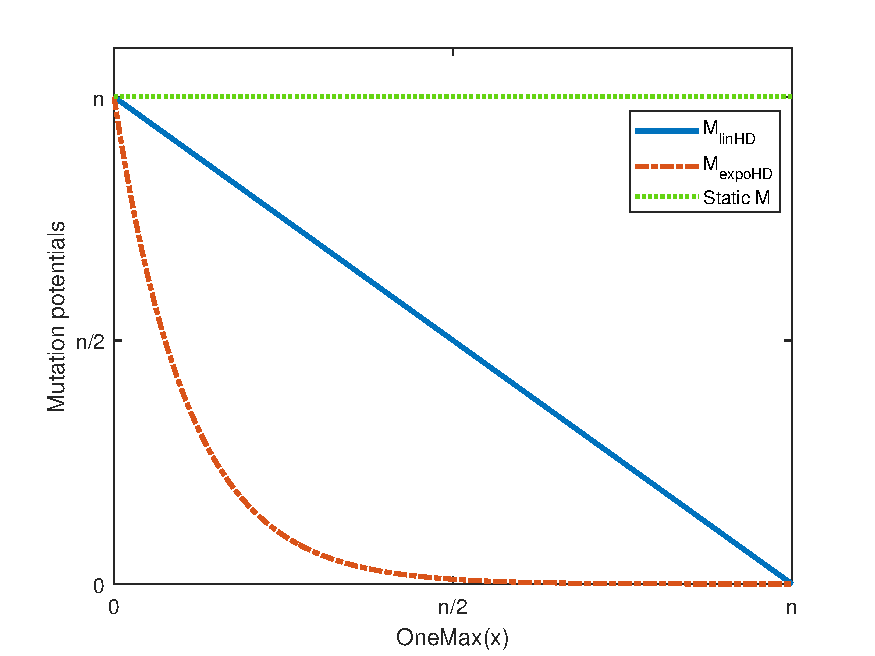
\includegraphics[width=1\textwidth]{a}
% \caption{Inversely proportional mutation potentials for \textsc{OneMax}.}
% \label{fig:onemax}
%\end{minipage}%
%\begin{minipage}{.5\textwidth}
%  \centering
%  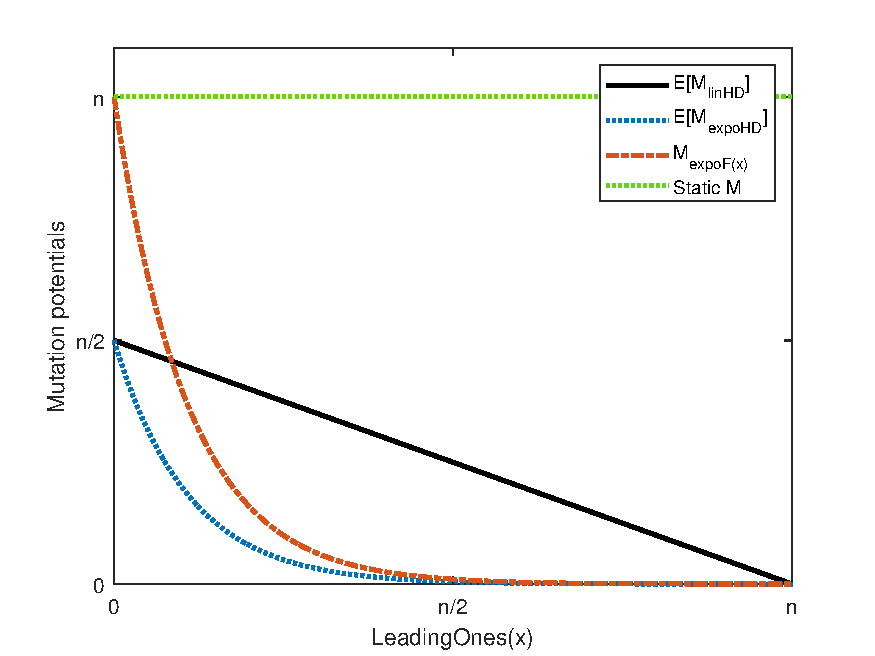
\includegraphics[width=1\textwidth]{b}
% \caption{Inversely proportional potentials for \textsc{LeadingOnes}. Expected values are shown for those using Hamming distance.}
% \label{fig:leadingones}
%\end{minipage}
%\end{figure}

In this section, we evaluate the performance of the three different \IPHfcm{} operators, %(1), (2) and (3),
assuming the optimum is known (i.e., best $=$ opt). Under this assumption, the operators exhibit their ideal behaviour (i.e., the mutation potential decreases with the desired rate as the optimum is approached).
Our aim is to evaluate what speed-ups can be achieved in ideal conditions compared to the well-studied static mutation potentials. To achieve such comparisons we perform runtime analyses of the (1+1)~IA  using the \IPHfcm{} on the standard \textsc{OneMax} and \textsc{LeadingOnes} unimodal benchmark functions for which the performance of the same algorithm using static mutation potentials is known~\cite{CorusOlivetoYazdani2019TCS}. The simple to define \textsc{OneMax} function counts the number of 1-bits in \new{a} bit string and is normally used to evaluate the hill climbing ability of algorithms~\cite{LehrTEVC2018,CorusOlivetoTEVCsteadyGA2017,CorusOlivetoAlgo2020,DoerrDoerrEbel2015}. On the other hand, \textsc{LeadingOnes} is a slightly harder unimodal problem which counts the consecutive number of 1-bits at the beginning of the bit string before the first 0-bit. 
Evolutionary algorithms using standard bit mutation (or k-bit flip local search mutation) optimise the functions respectively in $\Theta(n \log n)$ and $\Theta(n^2)$ expected fitness function evaluations \cite{DrosteJansenWegener2002,BoettcherEtAl2010,DoerrEtAl2016B,LissovoiOlivetoWarwicker2020,DLOW2018}, while static hypermutations are a linear factor slower\cite{CorusOlivetoYazdani2019TCS}.

While in practice both evolutionary algorithms and artificial immune systems use a population of solutions, in this paper we consider single trajectory algorithms to better highlight the performance of all the considered hypermutation operators.
The pseudo-code of a simple \new{immune algorithm,} the \oneoneIA{}, is given in Algorithm~\ref{alg:simple}. It simply uses one candidate solution in each iteration to which inversely proportional hypermutations are applied. For the function Hypermutate$(x)$, \IPHfcm{} performs two steps: 
1) it calculates the mutation potential $M$, and 2) it creates $y$ by flipping at most $M$ distinct bits of $x$ selected uniformly at random without replacement one after another until a constructive mutation happens. Otherwise it returns the last constructed solution. A  constructive mutation is a mutation step where the evaluated bit string is at least as fit as the parent \new{$x$}. 
%
The results proven in this section and comparisons with static hypermutations and the IPH operators from the literature are summarised in Table~\ref{table:afl}.


Before stating the main results, we first introduce the following lemma (the Ballot theorem) which is used throughout this paper to derive lower bounds on the expected runtime of the algorithms~\cite{feller1968,JansenZarges2011,CorusOlivetoYazdani2019TCS}.  This theorem is essentially used to show the probability of picking more 1-bits than 0-bits during one hypermutation operation given that there are more 1-bits in the initial bit-string (or vice-versa). 
%
\begin{lemma} [Ballot Theorem~\cite{feller1968}] \label{lem:ballot} 
In a ballot, suppose that candidate P receives $p$ votes and candidate Q receives $q$ votes such that $p>q$. The probability that throughout the counting P is always ahead of Q is $(p-q)/(p+q)$. 
\end{lemma}

{\color{blue}In the context of hypermutation operators, the vote counts are the initial number of $0$ and $1$-bits in the solutions, while counting the votes correspond to flipping them until the first constructive mutation. The probability that a constructive mutation is found is equivalent to the probability that the $q$ candidate having as many votes counted as the other during any time in the counting process.}

\begin{table}[t!]
\caption{Comparison of the expected runtimes obtained by different hypermutation schemes for \textsc{OneMax} and \textsc{LeadingOnes}. The original IPH operator of Opt-IA \cite{CutelloNicosiaPavoneTimmis2007}  has the same expected runtimes as the $(1+1)~$IA using static hypermutations \cite{JansenZarges2011}. \new{`$^*$' indicates that the result can be easily drawn from the analysis for \textsc{OneMax} \cite{Zarges2008}.}}
%The same result as $(1+1)~IA^{hype}$ using static hypermutation ($M=n$) has been shown for the original IPM of Opt-IA \cite{JansenZarges2011}.}
\begin{center}
\resizebox{\columnwidth}{!}{
	\begin{tabular}{ |l l l| }
		\hline
		\oneoneIA & \textsc{OneMax} &  \textsc{LeadingOnes} 
		\T\B \\ \hline
		
		Using static hypermutation & $\Theta(n^2\log n)$  \cite{CorusOlivetoYazdani2019TCS} & $\Theta(n^3)$ \cite{CorusOlivetoYazdani2019TCS}
		\T\B\\
		
		
		Using IPH of Clonalg & $e^{\Omega(n)}$ \cite{Zarges2008}  & ${e^{\Omega(n)}}^*$
		\T\B\\
		
		
		Using IPH of Opt-IA & $\Theta(n^2 \log n)$ \cite{JansenZarges2011}  & $\Theta(n^3)$ \cite{JansenZarges2011} 
		\T\B\\
		
		Using \IPHfcm{} with {\linHD } & $\Theta(n^2)$ & $\Theta(n^3)$
		\T\B\\ 
		Using \IPHfcm{} with \expoF & $O(n^{(3/2)}\log n)$, $\Omega(n^{3/2-2\epsilon})$ & $O(n^3/\log n)$, $\Omega(n^{5/2+\epsilon})$
		\T\B \\
		Using \IPHfcm{} with \expoHD & $O(n^{(3/2)}\log n)$, $\Omega(n^{3/2-2\epsilon})$ & $O(n^{\frac{5/2+\epsilon}{\ln n}})$, $\Omega(n^{9/4-\epsilon})$
		\T\B \\
		
		% $(1+1)$~IA using \blin & $\Theta(n \log n)$ & $\Theta(n^2)$
		% \T\B \\
		% $(1+1)$~IA using \bexpo & $\Theta(n \log n)$ & $\Theta(n^2)$
		%\T\B \\
		% Fast $(1+1)$~IA$_{\beta}$ & $O(n \log n)$ & $O(n^2)$
		% \T\B \\
		
		\hline
	\end{tabular}
}
\end{center}
\label{table:afl}
\end{table}




%
%In the mutation potential formulas, $best$ can be defined according to different strategies, e.g., it can be an estimation of the best individual or the best individual seen so far. As we ideally want to mutate inversely proportional to the optimum, in this section we assume the optimum is known and hence $best$ is the global optimum. By this assumption, we can see more clearly how the mutation operator behaves.
%
%A simple framework to analyse different inversely proportional mutation potentials is shown in %Algorithm \ref{alg:simple}. 



%\begin{algorithm} 
%    \caption{\oneoneIA}
%   \begin{algorithmic}[1] % The number tells where the line numbering should start
%           \STATE{Initialise $x \in\{0,1\}^n$ uniformly at random;}
%          \STATE Evaluate $f(x)$;      
%          \WHILE{termination condition is not satisfied} %\Comment{}  
%          \STATE{Choose $M \in \{ M_{linHD},M_{expoF(x)},M_{expoHD}\} $};
%          %\STATE{$y \leftarrow invHyp(x)$}
%          \STATE{$y:=x$};
%         \STATE{Flip at most $M$ distinct bits of $y$ selected uniformly at random one after another until a \textit{constructive mutation} happens;};
%			\IF {$f(y) \geq f(x) $}
%			\STATE{$x:=y$}.
%			\ENDIF
%         \ENDWHILE
%   \end{algorithmic} \label{alg:simple}
%\end{algorithm}

%\begin{algorithm}[t] 
%    \caption{\oneoneIA}
%    \begin{algorithmic}[1] % The number tells where the line numbering should start
%            \STATE{Initialise $x \in\{0,1\}^n$ uniformly at random;}
%            \STATE evaluate $f(x)$;      
%            \WHILE{termination condition is not satisfied} %\Comment{}  
%            \STATE{ $M := IPM(x) $};
%            %\STATE{$y \leftarrow invHyp(x)$}
%            \STATE{create $y$ by flipping at most $M$ distinct bits of $x$ selected uniformly at random one after another until a \textit{constructive mutation} happens};
%			\IF {$f(y) \geq f(x) $}
%			\STATE{$x:=y$}.
%			\ENDIF
%            \ENDWHILE
%    \end{algorithmic} \label{alg:simple}
%\end{algorithm}


\begin{algorithm}[t] 
\caption{\oneoneIA}
\begin{algorithmic}[1] % The number tells where the line numbering should start
\STATE{Initialise $x \in\{0,1\}^n$ uniformly at random;}
\STATE Evaluate $f(x)$;      
\WHILE{termination condition is not satisfied} %\Comment{}  
{\color{blue}
\STATE Update mutation potential $M$;  
\STATE{ $y:=$ Hypermutate$(x, M)$};}
%\STATE{$y \leftarrow invHyp(x)$}
%\STATE{create $y$ by flipping at most $M$ distinct bits of $x$ selected uniformly at random one after another until a \textit{constructive mutation} happens};
\IF {$f(y) \geq f(x) $}
\STATE{$x:=y$}.
\ENDIF
\ENDWHILE
\end{algorithmic} \label{alg:simple}
\end{algorithm} 

\begin{algorithm}[t]

	\caption{\textsc{Hypermutate}$(x,M)$}
	\begin{algorithmic}[1]
{\color{blue}
		\STATE $y \gets x$;
		\FOR{$i = 1$ \textbf{to} $M$}
		\STATE Flip one previously unflipped bit of $y$ chosen uniformly at random;
		\STATE Evaluate $f(y)$;
		\IF{$f(y) \geq f(x)$}        
		\STATE \textbf{return} $y$;
		\ENDIF
		\ENDFOR
		\STATE \textbf{return} $y$;     
	}
	\end{algorithmic}
	\label{alg:hypermutate}
\end{algorithm}


\subsection{Performance for \textsc{OneMax} in Ideal Conditions}
\begin{figure}[t!]
\centering
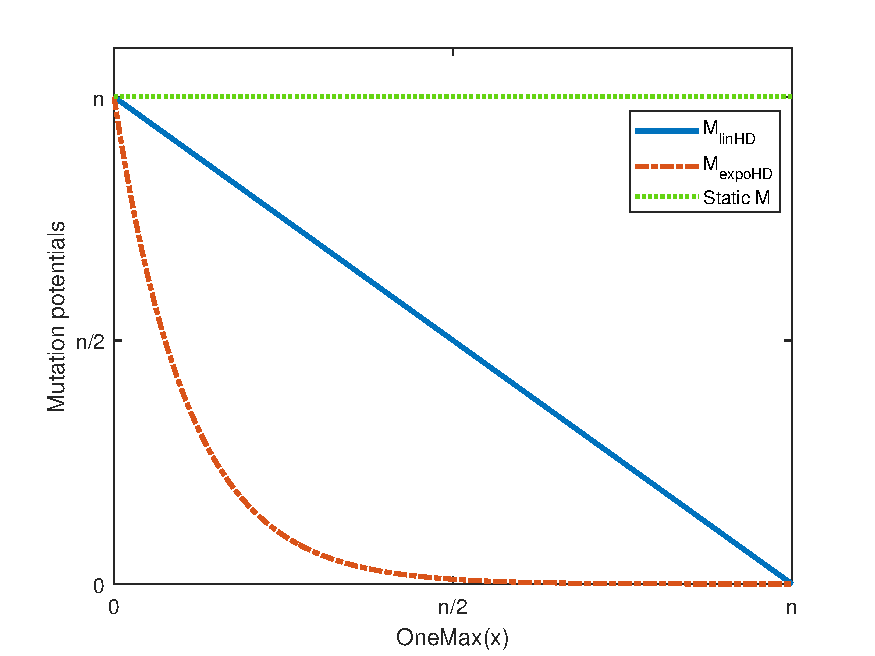
\includegraphics[width=\columnwidth]{a}
\caption{Static and inversely proportional mutation potentials for \textsc{OneMax}.}
\label{fig:onemax}
\end{figure}

The following theorems derive the expected runtimes using each of the three IPH operators for the function $\textsc{OneMax}(x):=\sum_{i=1}^{n}x_i$. 
Figure \ref{fig:onemax} %and \ref{fig:leadingones} 
shows how the studied mutation potentials ideally decrease during the run of the algorithm when optimising the function. 
Notice that for \textsc{OneMax} the behaviours of   {\expoF } and {\expoHD }  are the same. %\textsc{OneMax} and \textsc{LeadingOnes}, respectively. 
By decreasing the potential linearly with the decrease of the Hamming distance, a logarithmic factor may be shaved off from the expected runtime of the {\oneoneIA } compared to the expected runtime achieved by the same algorithm using static hypermutation potentials.



\begin{theorem} \label{th:linHD-OM}
The {\oneoneIA } using \IPHfcm{} with {\linHD } optimises \textsc{OneMax} in $\Theta(n^2)$ expected fitness function evaluations.
\end{theorem}

\begin{proof}
Considering $i$ as the number of 0-bits in the candidate solution, the probability of improvement in the first step is $i/n$. Knowing that at most $n$ improvements are needed to find the optimum and in case of failure, $H(x,\text{opt})=i$ fitness function evaluations would be wasted, the total expected time to optimise \textsc{OneMax} is at most $\sum_{i=1}^n \frac{n}{i} \cdot i =O(n^2)$.

For the lower bound, we use the Ballot theorem (Lemma~\ref{lem:ballot}). 
\new{We flip at most $M \le n$ bits, and the probability that an improvement happens is the probability that at some moment there will be at least as many flipped zeros as there are flipped ones. So pessimistically we can assume that  $M = n$ bits are always flipped, since it maximizes the chances of this unfortunate event.} 

By Chernoff bounds, the number of 0-bits in the initialised solution is at least $n/3$ w.o.p. Considering the number of 
0-bits as $i=q$ and the number of 1-bits as $n-i=p$, the probability of 
an improvement is at most $1-(p-q)/(p+q)=1-(n-2i)/n=\frac{2i}{n}$ by the Ballot theorem, where $i=H(x, opt)$. This means that we need to wait at least $\frac{n}{2i}$ iterations to see an improvement and each time the mutation operator fails to improve the fitness {(\color{blue}$\frac{n}{2i} - 1$ times in expectation) }, $i$ fitness function evaluations will be wasted. Considering that at least $n/3$ improvements are needed, the expected time to optimise \textsc{OneMax} is larger than $\sum_{i=1}^{n/3} {\color{blue}\left(\frac{n}{2i}-1\right)} \cdot i= \Omega(n^2)$.
\end{proof}

The following theorem shows that a greater speed up may be achieved if the potential decreases exponentially rather than linearly. Note that for \textsc{OneMax} the Hamming distance of a solution to the optimum and its difference in fitness are the same. %The proof is omitted due to lack of space.
% Hence, the subsequent corollary is obvious.
\new{Hence, there is no difference between the behaviours of the algorithm when using $M_{expoF(x)}$ and $M_{expoHD}$.} 
Figure \ref{fig:onemax} highlights the reason why these operators waste fewer fitness evaluations.

\begin{restatable}{theorem}{expofx} \label{cor:omexpohd}
The {\oneoneIA } using IPH with either {\expoF } or {\expoHD } optimises \textsc{OneMax} in $O(n^{3/2} \log 
n)$ and $\Omega(n^{3/2-\epsilon})$ expected fitness function evaluations for 
any arbitrarily small constant $\epsilon>0$.
\end{restatable}
%\end{theorem}

\begin{proof}
We prove the results for \expoF{} which applies to \expoHD{} as well. 
To prove the upper bound, we use that by Chernoff bounds the initialised solution has at most $n/2+ n^{2/3}$ 0-bits w.o.p. {\color{blue} If this event fails, we will assume that the mutation potential is always $M=n$ which still yields polynomial runtime following the same arguments below and contributes a $o(1)$ to the total expected time}. The probability of improvement in the first mutation step is at least $i/n$ with $i$ being the number of 0-bits. As we need at most $n/2+n^{2/3}$ improvements and each time the mutation fails to make an improvement at most $n^{1-\frac{n-i}{n}}$ fitness function evaluations are wasted, the total expected time to find the optimum is $E(T) \leq o(1) + \sum_{i=1}^{n/2+n^{2/3}} \frac{n}{i} \cdot n^{\frac{i}{n}}= O (n^{3/2} \log n)$ by pessimistically assuming $i=n/2+n^{2/3}$ in $n^{i/n}$ {\color{blue} which yields $n^{1/2+n^{-1/3}}=\sqrt{n} \cdot e^{\frac{\ln n}{n^{1/3}}}=\sqrt{n} \cdot e^{o(1)}=O(\sqrt{n})$}.

To prove the lower bound, we again consider $i$ as the number of 0-bits. By Chernoff 
bounds, $i$ is at least $n/2-\epsilon n$  in the initialised bit string for some arbitrarily small constant $\epsilon>0$. 
The probability of improvement is at most $2i/n$ by the Ballot theorem, and the number of wasted fitness function evaluations at each failure is 
$n^{\frac{i}{n}}$. {\color{blue} Since our operator cannot improve the \textsc{OneMax} function value more than one due to FCM,} when we consider the time spent between levels $n(1/2 + 
\epsilon/2)$ and $n(1/2+\epsilon)$, we get the expected time of 
{\color{blue}$n^{\frac{n/2-\epsilon n}{n}} \cdot \sum_{k=n/2+n\epsilon/2 }^{n/2+\epsilon 
n} \frac{n}{2(n-k)}-1 \geq \sum_{k=n/2+n\epsilon/2 }^{n/2+\epsilon 
n} \frac{\epsilon}{1-\epsilon}=n^{1/2-\epsilon} \cdot \epsilon n/2 \cdot \frac{\epsilon}{1-\epsilon}= 
\Omega(n^{3/2-\epsilon})$.}
\end{proof}

{\color{blue}Here, we note that even though we picked the $\epsilon$ to be a constant, the leading term in the lower bound depends on $\epsilon$ quadratically which might impact practical applications.}



%\begin{corollary}\label{cor:omexpohd}
%The {\oneoneIA } using {\expoHD } optimises \textsc{OneMax} in $O(n^{3/2+\epsilon} 
%\log 
%n)$ and $\Omega(n^{3/2-\epsilon})$ expected fitness function evaluations for 
%any arbitrarily small constant $\epsilon>0$.
%\end{corollary}

%\begin{proof}
%This proof is exactly similar to the proof of Theorem \ref{th:expoF(x)-UPonOM}.
%% except that here the maximum number of wasted fitness function evaluations is different. Considering that in case of failure in improving the fitness in the first step $n^{HD/n}$ fitness function evaluations will be wasted, the total expected time to optimise \textsc{OneMax} is at most $E(T) \leq \sum_{i=1}^{n/2+\epsilon n} \frac{n}{i} \cdot n^{\frac{i}{n}}= O(n^{3/2+\epsilon} \log n)$. {\color{red} $O(n^2 \log{n})$ seems to be the order of the sum since $n^{1-i/n}<n$}.
%\end{proof}

%\begin{theorem}
%The \oneoneIA using mutation potential \expoHD optimises \textsc{OneMax} in $\Omega(n^{3/2-2\epsilon})$ expected fitness function evaluations.
%\end{theorem}

%\begin{proof}
%Similar to the proof of theorem \ref{th:expoF(x)-LBofOM}.
%%  $\sum_{i=1}^{n/3} \frac{n}{2i} \cdot n^{i/n}= ?$. {\color{red} While $i\in \{1,\ldots,n/3\}$, $n^{1-i/n}\in[n^{1-1/n},n^{2/3}]$. If we sum over this interval we can only get $n\cdot n \cdot n^{2/3}=\Omega(n^{8/4})$. I suggest analysing the expected runtime of the last $\epsilon n$ steps to get a $\Omega(n^{3-\epsilon})$ result, for any arbitrarily small constant $\epsilon$.}
%\end{proof}


\subsection{Performance for \textsc{LeadingOnes} in Ideal Conditions}
\begin{figure}[t!]
\centering
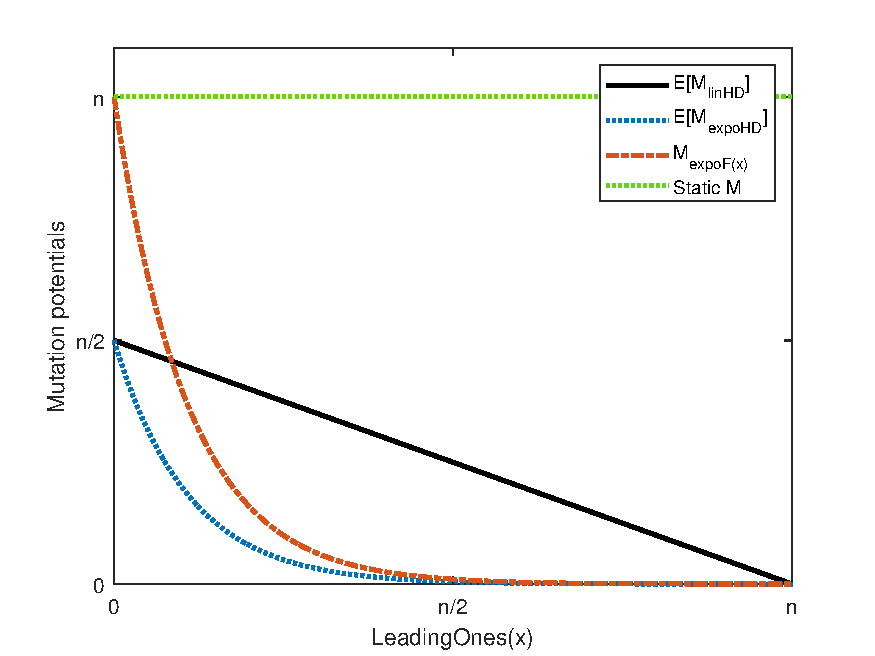
\includegraphics[width=\columnwidth]{b}
\caption{Static and inversely proportional  mutation potentials for \textsc{LeadingOnes}. Expected values are shown for those using Hamming distance.}
\label{fig:leadingones}
\end{figure}

In the previous subsection, it was shown that decreasing the mutation rate linearly with the Hamming distance to the optimum allows for a logarithmic factor speed-up for \textsc{OneMax} compared to using  static hypermutations. The following theorem shows that no asymptotic improvement over static mutation potentials is achieved for \textsc{LeadingOnes}$:= \sum_{i=1}^{n}\prod_{j=1}^{i}x_i$. The main reason for the lack of improvement is that a linear mutation potential is sustained until at least a linear number of improvements are achieved.


%{\color{red}(can we still use the same expectation for free riders?)}
\begin{theorem} \label{th:linHD-LO}
The {\oneoneIA } using \IPHfcm{} with {\linHD } optimises \textsc{LeadingOnes} in $\Theta(n^3)$ expected fitness function evaluations.
\end{theorem}

\begin{proof}
%The probability of improvement in each step is at least $1/n$ which is the probability of flipping the leftmost 0-bit. As at most $n$ improvements are needed and each failure in improvement yields $\frac{n-i-1}{2}+1+\epsilon n$ wasted fitness function evaluations in expectation (i.e., the expected $H(x,opt)$ value), the expected time to find the optimum is at most $\sum_{i=1}^n n \cdot \left(\frac{n-i-1}{2}+1+\epsilon n\right)= O(n^3)$.

The proof for the lower bound follows that of Theorem 3.6 in \cite{CorusOlivetoYazdaniGECCO2017} for the expected runtime of the $(1+1)$~IA %$_{\geq}$\footnote{$(1+1)$~IA$_{\geq}$ is a \oneoneIA{} whose  selection mechanism accepts equally fit solutions.}
using static hypermutation with potential $M:=cn$ with the exception that the amount of wasted fitness function evaluations in case of failure at finding an improvement within a hypermutation is now $H(x,\text{opt})$ instead of $cn$.


Considering $i$ as the number of leading 1-bits, we denote the expected number of fitness function evaluations until an improvement happens by $E(f_i)$. Any such candidate solution has $i$ leading 1-bits with a 0-bit following, and then $n-i-1$ \emph{trailing bits}. The trailing bits stay uniformly distributed throughout the run since the hypermutation operation can only terminate with an accepted solution by immediately flipping the leftmost $0$-bit, which does not alter the trailing bits, or by immediately flipping a random trailing bit, which does not affect the probability of the flipped position being 1 or 0 after it is flipped\cite{DrosteJansenWegener2002}.   We take into account three possible events $E_1$, $E_2$ and $E_3$ that can happen in the first bit flip: $E_1$ is the event of flipping a leading 1-bit which happens with probability $i/n$ {\color{blue} and allows the hypermutation to keep flipping $M-1$ more bits }, $E_2$ is the event of flipping the first 0-bit which happens with probability $1/n$, and $E_3$ is the event of flipping any other bit which happens with probability $(n-i-1)/n$. {\color{blue}Since FCM stops the hypermutation operator as soon as an equally fit solution is sampled $E_2$ and $E_3$ each stops the hypermutation operation.} So we get $E(f_i|E_1)=H(x,opt)+ E(f_i)$, $E(f_i|E_2)=1$, and $E(f_i|E_3)=1+ E(f_i)$. Hence, by the law of total expectation, the expected number of fitness function evaluations for every improvement is $ E(f_i) = \frac{i}{n} \left( H(x,opt)+ E(f_i)\right) + \frac{1}{n} \cdot 1 +\frac{n-i-1}{n} \left( 1+ E(f_i)\right)$. Solving the equation for $E(f_i)$ gives us $E(f_i)=
%\frac{in-i^2-i-i\epsilon n}{2}
i\cdot H(x,opt)+n-i\geq i\cdot H(x,opt) $. Since the bits after the leftmost 0-bit are distributed uniformly at random \cite{DrosteJansenWegener2002}, {\color{blue} while there are still a linear number of trailing bits} the value of $H(x,opt)$ is not less than $1+ \frac{(n-i-1)}{2}- \frac{\epsilon }{2}n$ w.o.p. by Chernoff bounds. Thus, we conclude $E(f_i) \geq \frac{(1-\epsilon)in-i^2+i}{2}\cdot {\color{blue}(1-o(1))}$. The right hand side of the inequality has a second derivative of $-2$ with respect to $i$, and therefore it is concave. For the interval $i\in [n/2-\epsilon^*n, n/2+\epsilon^*n]$ its value is of order $\Omega(n^2)$ for some   arbitrarily small $\epsilon^*>0$.


As we are computing the lower bound, we have to take into account the probability of skipping any level $i$. To do this, we need to calculate the expected number of consecutive 1-bits that follow the leftmost 0-bit (called free riders \cite{DrosteJansenWegener2002}). The expected number of free riders is $\sum_{i=1}^{n-i-1} i \cdot 1/2^{i+1} < \frac{1}{2} \cdot \sum_{i=0}^{\infty} i \cdot (1/2)^i= \frac{1}{2} \cdot \frac{1/2}{(1-1/2)^2}=1$. This means that {\color{blue}$p^{*}_{i}$}, the probability of not skipping a level $i$ is $\Omega(1)$.
%We know that the expected number of consecutive 1-bits that follow the leftmost 0-bit is less than two \cite{DrosteJansenWegener2002} which means the probability of not skipping a level $i$ is $\Omega(1)$.
On the other hand, with probability at least $1- 2^{-n/3}$, the initial solution does not have more than $n/3$ leading 1-bits. Thus, we obtain a lower 
bound of  $(1-2^{-n/3}) \sum_{i=n/2-\epsilon^*n}^{n/2+\epsilon^*n} p^{*}_{i}\cdot E(f_i)=\Omega(1) \sum_{i=n/2-\epsilon^*n}^{n/2+\epsilon^*n} \frac{in-i^2+i-i\epsilon n}{2}=\Omega(n^3)$ on the expected number of fitness function evaluations.

Now we prove the upper bound. The probability of improvement in each step is at least $1/n$ which is the probability of flipping the leftmost 0-bit {\color{blue} in the first} bit-flip. Since at most $n$ improvements are needed and each failure at improving yields {\color{blue} at most $n$} wasted fitness function evaluations, the expected time to find the optimum is at most $\sum_{i=1}^n n \cdot {\color{blue}n}= O(n^3)$.

\end{proof}


Theorem \ref{expohdOnLO} shows that the exponential fitness-based mutation 
potential provides at least a logarithmic and at most a $\sqrt 
n$ factor speed-up compared to static mutation potentials. Before proving the main results, we introduce the following  lemma that will be used in the proof of the upcoming theorems.
\begin{lemma}\label{lem:expo}
For large enough $n$ and {\color{blue}any arbitrary constant} $\epsilon$, 
$n^{1/n^{\epsilon}}= (1+\frac{\ln{n}}{n^{\epsilon}})(1 \pm o(1))$.
\end{lemma}
\begin{proof}
	$n^{\frac{1}{n^\epsilon}} = e^{\frac{\ln(n)}{n^\epsilon}} = 1 + \frac{\ln(n)}{n^\epsilon} + o(\frac{\ln(n)}{n^\epsilon})$ by the Taylor's series of the exponent.
	
\end{proof}


\begin{theorem} \label{expohdOnLO}
The {\oneoneIA } using \IPHfcm{} with {\expoF } optimises \textsc{LeadingOnes} in $O(n^3/\log n)$ and 
$\Omega(n^{(5/2)-\epsilon})$  expected fitness function evaluations for any 
arbitrarily small constant $\epsilon>0$. 
\end{theorem}

\begin{proof}
{\color{blue} The expected number of leading 1-bits is smaller than 1 in the initialised bit 
	string since each bit 0 or 1 with $1/2$ probability and $\sum^{n}_{i=1}2^{-i}<1$ for finite $n$.} The expected number of leading 1-bits is smaller than 1 in the initialised bit 
string. The probability of improvement in the first step {\color{blue} of the hypermutation} is $1/n$. In the case of 
failure at improving in the first step, at most $n^{\frac{n-i}{n}}$ fitness 
function evaluations are wasted where $i$ is the number of leading 
1-bits. {\color{blue}$\sum_{i = 0}^{n - 1} n \cdot n^{(n - i) / n} < n^2 \sum_{i = 0}^{+\infty}(n^{-1/n})^i = n^2 \cdot \frac{1}{1 - n^{-1/n}} = n^2 \cdot \frac{n^{1/n}}{n^{1/n} - 1} = n^2 \cdot \frac{1 + o(1)}{\frac{\ln{n}}{n} + o(\frac{\ln{n}}{n})} = O(\frac{n^3}{\log{n}})$. }

Therefore, the total expected time to find the optimum is  $E(T) \leq 
\sum_{{\color{blue}i=0}}^{n-1} n \cdot n^{(n-i)/n}=O( n^3/\log n)$ considering that $ 
\sum_{{\color{blue}i=0}}^{n-1} n^{i/n}= \sum_{{\color{blue}i=1}}^n (n^{1/n})^{i-1}=\frac{1-n}{1-n^{1/n}}$ (using the general partial power series sum: $\sum_{i=0}^{m}a^{i}=\frac{1-a^{m+1}}{1-a}$ for $a\neq 1$)  that gets in turn bounded from above by $n^2/(\log n)$ using Lemma~\ref{lem:expo}.


The proof of the lower bound is similar to the proof of Theorem \ref{th:linHD-LO}, except for the calculation of $E(f_i)$ when we want to consider the amount of wasted fitness function evaluations in case of $E_1$ happening. Here we have $ E(f_i) = \frac{i}{n} \left( n^{(n-i)/n}+ E(f_i)\right) + \frac{1}{n} \cdot 1 +\frac{n-i-1}{n} \left( 1+ E(f_i)\right)$. Solving it for $E(f_i)$ gives us $E(f_i)=i\cdot n^{(n-i)/n}+n-i$. 
{\color{blue}Following the proof of Theorem~\ref{th:linHD-LO}}, the expected time to optimise \textsc{LeadingOnes} is 
$(1-2^{-n/2})\sum_{i=n/2}^{n} {\color{blue}p_{i}^{*}} E(f_i)=\Omega(1) \sum_{i=n/2}^{n} 
\left(i\cdot n^{(n-i)/n}+n-i \right)=\Omega(1)\left( \sum_{i=n/2}^{n} (n-i)+ 
\sum_{i=n/2}^{n} \left(i\cdot n^{(n-i)/n}\right)\right)$. Evaluating the second 
sum in the interval $i\in [n/2+\frac{\epsilon n}{2}, n/2+\epsilon n]$, we get $\epsilon 
n/2 \cdot (n/2 + \epsilon n)  \cdot 
n^{1/2-\epsilon/2}=\Omega(n^{5/2-\epsilon})$.
%{\color{red} For $i\in\{n(1-\epsilon),\ldots,n\}$, $i n^{i/n}=\Omega(n n^{1-\epsilon})$ for any arbitrarily small constant $\epsilon$. If sum over $\epsilon n$ levels we can get $\Omega(n^{3-\epsilon})$ }
\end{proof}

An advantage of Hamming distance-based exponential decays of the mutation potential
compared to fitness-based ones is provided by the following theorem for \textsc{LeadingOnes}.
The reason can be seen in Figure \ref{fig:leadingones}.  While the initial fitness is very low, the potential is very high, but the actual number of bits that have to be flipped to reach the optimum (i.e., the Hamming distance), is much smaller. More precisely, fitness-based potentials suggest to flip $n$ bits when only $n/2$ bits have to be flipped in expectation to reach the optimum in one step. 
{\expoHD } exploits this property, thus wastes fewer fitness evaluations than \expoF. 
%The proof of the following theorem is similar to that of the two previous theorems and is omitted due to lack of space.
% the initial Hamming distance for the \textsc{LeadingOnes} is roughly $n/2$ the fitness difference with the optimum is $n$, leading to linear initial potential instead of $\Theta(n^{1/2})$.

\begin{restatable}{theorem}{expohdLO}\label{thm:expohdLO}
The {\oneoneIA } using \IPHfcm{} with {\expoHD } optimises \textsc{LeadingOnes} in 
$O(\frac{n^{5/2+\epsilon}}{\ln n})$ and $\Omega(n^{9/4-\epsilon})$ expected 
fitness function evaluations for any arbitrarily small constant $\epsilon>0$. 
\end{restatable}

\begin{proof}
	
	$$ n^{-1/(2n)} ;\ge; \bigl(1-\tfrac{\ln n}{2n}\bigr)\bigl(1-o(1)\bigr), $$ 
	
The proof for the upper bound is similar to the proof of Theorem~\ref{th:linHD-LO}, however, each 
failure in improvement yields $n^{H(x, \text{opt})/n}$ wasted fitness function evaluations. 
Since the bits after the leading ones are uniformly distributed, by Chernoff bounds the number 
of 0-bits (Hamming distance to the optimum) is smaller than  $1+(n-i-1)/2+\epsilon n$ 
w.o.p. {\color{blue}Considering that the runtime will be polynomial even when the number of $0$-bits is larger than $1+(n-i-1)/2+\epsilon n$}, the expected time to optimise \textsc{LeadingOnes} is ${\color{blue}o(1)}+\sum_{i=1}^{n} n \cdot 
n^{\frac{1+(n-i-1)/2+\epsilon n}{n}}= {\color{blue}o(1)}+n \sum_{i=1}^{n} 
n^{\frac{1}{2}-\frac{i}{2n}+\epsilon+\frac{1}{2n}}={\color{blue}o(1)}+n \cdot n^{\frac{1}{2}+\epsilon+\frac{1}{2n}} \sum_{i=1}^{n} 
n^{-\frac{i}{2n}}$. Knowing that 
$\sum_{i=0}^{\infty}n^{-\frac{i}{2n}}=\frac{1}{1-n^{\frac{-1}{2n}}}=${$\color{blue} \frac{n^{\frac{1}{2n}}}{n^{\frac{1}{2n}} - 1} = \frac{1 + o(1)}{\frac{\ln{n}}{2n} + o\left(\frac{\ln{n}}{2n}\right)} = O\left(\frac{n}{\log{n}}\right)$ where in the third equality we used Taylor expansion of the exponential function.}  Hence, the expected time is $E(T) 
< {\color{blue}o(1)}+n^{\frac{3}{2}+\epsilon} \cdot n^{\frac{1}{2n}} \cdot O\left(\frac{n}{\log n}\right)=O\left(\frac{n^{\frac{5}{2}+\epsilon}}{\log n}\right)$.



The proof of the lower bound is also similar to the proof of Theorem~\ref{th:linHD-LO}. 
By taking the same steps and solving the equation for $E(f_i)$,we get
$E(f_i){\color{blue}\ge} i \cdot n^{\frac{1}{n}+\frac{n-i-1}{2n}-\epsilon}+n-i$. Then, by taking into account the probabilities of starting with fewer than $n/2$ leading 1-bits and skipping a level $i$, we get the expected runtime of 
\begin{align*}
&(1-2^{-n/2})\sum_{i=n/2}^{n} {\color{blue}p_{i}^{*}} \cdot E(f_i)\\
&\geq \Omega(1) \sum_{i=n/2+\epsilon 
	n/2}^{n/2+\epsilon n} 
\left( i n^{1/n+((n-i-1)/2n)-\epsilon}+n-i )\right)\\
&\geq \Omega(1) \sum_{i=n/2+\epsilon 
	n/2}^{n/2+\epsilon n}  in^{1/2-\epsilon+(1/(2n))-(i/(2n))}= \Omega(n^{(9/4)-\epsilon}).
	\end{align*} 
\end{proof}


%where  \textsc{ZeroMax(x)} counts the number of 0-bits in the bit string. 

%\subsection{Ridge}

%\begin{equation*}
%\textsc{Ridge}(x):= \begin{cases}
%		kn+n  & \text{if}\; x=1^k0^{n-k},\; \text{for}\; 0\leq k \leq k_{max}\\
%        \textsc{ZeroMax(x)} & \text{otherwise},
% \end{cases}
%\end{equation*}


%
%The reason we look at \textsc{Ridge} is that the distance to the optimum starts from nearly $n$ (unlike \textsc{LeadingOnes}). It is an example where the whole range of mutation rates occurs. However, giving that the global optimum is the opposite of the local optimum, hypermtations can easily flip everything and find it in one step after reaching local optima. That is why we use the truncated version of \textsc{Ridge}.
% \begin{figure}[t!]
% \centering
%  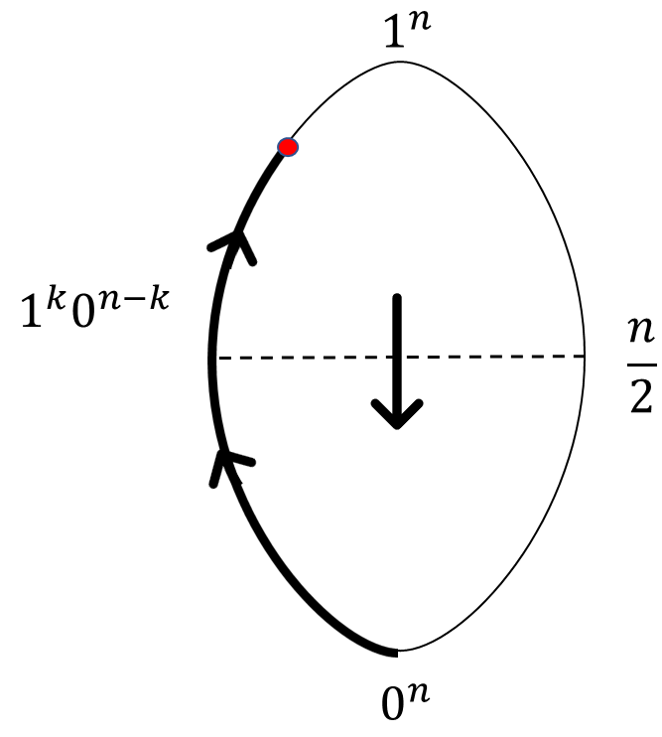
\includegraphics[width=0.15\textwidth]{ridge}
% \caption{\textsc{Ridge}}
% \label{fig:plot}
% \end{figure}
%
%
%\begin{theorem} \label{th:linHDonRidge}
%The \oneoneIA using mutation potential \linHD optimises \textsc{Ridge} in $O(n^2 \log{n} + n\cdot k^2_{max})$ expected fitness function evaluations.
%\end{theorem}
%{\color{red}Do we need the lower bound for Ridge? it is very difficult to prove a lower bound for it}
%\begin{proof}
%
%%\item Jumping in the path: the problem of any jump of size 2 in the path is $O(1/n^2)$ ( $1/n^2+1/n^3+...$).
%By Chernoff bound, the initialised solution has at least 
%$n/2-\epsilon n$ 0-bits for any $\epsilon=\Theta(1)$ w.o.p.
%and is not a path point with probability $n/2^n$. 
%% We should also compute the probability of not finding any path point in every level $i$. we are $n/2-\epsilon n$ away from any path points (like the claim in the initialisation). 
%
%We pessimistically consider that an improvement can only be achieved in the 
%first mutation step of a hypermutation operation. Given that a path point is 
%not discovered before, with probability $i/n$ (where $i$ is the number of 
%1-bits in the bitstring of the current solution) we observe an improvement 
%in the
%\textsc{ZeroMax} value towards $0^n$, which is the first point of the path.  
%Considering that the Hamming distance to the optimum (i.e., $1^{k_{max}}0^{n-k_{max}}$) can be as large as $n$ during the progress towards $0^n$, in at most 
%%$\sum_{i=1}^{n} \frac{n}{i} \cdot (n-i)= O(n^2 \log n)$.
% $\sum_{i=1}^{n/2-\epsilon n} \frac{n}{i} \cdot n= O(n^2 \log n)$  the path will be found. After finding a point on the path, with probability 
%at least $1/n$ the leftmost 0-bit will get flipped in the first move and the 
%next path point will be discovered. Given that the current path 
%solution has $k$ 1-bits in its prefix, the hypermutation wastes $k_{max}-k$ 
%fitness function evaluations if it cannot improve the fitness value of the 
%current solution. Thus, total expected number of fitness function evaluations 
%is:
%\begin{align*}
%%  \[
% E[T] &\leq O(n^2 \log{n})+\sum\limits_{k=1}^{k_{max}} n \cdot \left( k_{max}-k 
%\right)   \\
%&\leq O(n^2 \log{n})+n\cdot \sum\limits_{k=1}^{k_{max}}  k_{max} -n 
%\sum\limits_{k=1}^{k_{max}}  k \\
%&\leq O(n^2 \log{n})+n\cdot   k^2_{max} -n \frac{k_{max} (k_{max}+1)}{2}\\
%&=O(n^2 \log{n} + n\cdot k^2_{max})
%% \]
%\end{align*}
%
%
%%number of wasted 
%%evaluations in case of failing to improve the individual in the first mutation 
%%step at most $i$ fitness function evaluation would be wasted, the expected time 
%%to find the optimum from the path is $\sum_{i=1}^n n \cdot i=O(n^3)$, which 
%%dominates the $O(n^2)$ expected time of first part. 
%
%%For Lower bound our approach is based on how many bits we sample at each level $i$ of the search space, and how many we can hit in the path. 
%% The probability of jumping to the path is actually very small overall. It is symmetric though, the same when $i$ is big and when $i$ is small. Being at every level $k$, the probability of hitting a path point is $\{\binom{n}{k}\}^{-1}$.(What we want at the end, is to see the probability of finding path points with $n^\epsilon \leq k \leq n/2$). \\
%%$Prob\{X_{ijk}:$ the probability that the $j$th mutation step starting from $i$th solution sampled on level $k$ is a path solution$\}$\\
%%Given that we are not improving zeromax, we are going back (any upper levels):$Prob\{X_{ijk} \in path\}=\sum_{l=k}^{n/2+\epsilon n} Prob\{X_{ijk}|X_{ijk}\in l\} \cdot Prob\{X_{ijk}\in 2^{\-\Omega(n^{\epsilon}}\}=\binom{n}{l}^{-1}$ . Now, since the biggest $l$ is $k$, this  probability is smaller than $\sum_{n/2}\binom{n}{k}^{-1}\cdot 1$ knowing that each time we add $n$. ($j->n$ steps, $i->$ at most $n$ solutions). 
%
%%Lower bound:By Chernoff bound, the initialised solution has $n/2-\epsilon n$ 0-bits w.o.p. for an arbitrary small $\epsilon=\Theta(1)$ and is not in the path with probability $1-n/2^{-n/2}$. Indicating the number of 1-bits with $i$, while $i$ is linear the probability of mutating to a bit string in the path is is exponentially small:
%%\begin{equation*}
%%n \cdot \binom{n}{\Theta(n)}^{-1}
%%\end{equation*}
%
%%Since all the number of possible bit strings in level $i$ decreases by decreasing $i$ (i.e., the denominator), the probability of finding a path point would be larger when $i$ is logarithmic constant. While the probability of improving on \textsc{ZeroMax} is $i/n$, what happens in the last step? with probability 1 we will find the path rather than all 0 bit string. Something seems wrong here.
%
%% Hence, jumping to the optimum has exponentially small probability as it is the probability of selecting almost $n/2$ 0-bits and nothing else. The individual will follow the \textsc{ZeroMax} gradient with probability at most $2i/n$ by Ballot theorem. Now what is the probability of reaching $0^n$ and not jumping to the path? The more we go towards the all 0 bit string, the higher the probability of jumping will be (%Jumping before reaching the $0^n$ to the path: conditional probability on not discovering the path at $k$  will be found by bounding $Bin(n,1/2)+2Bin(k,1/2)-k$).
%%If it reaches the all 0 bit string, then with probability at least $1/n$, which is the probability of flipping the right most 0, the optimum will be found in one step. If it is more probable to jump to the path rather than reaching all 0 bit string, then the proof will be different.
%\end{proof}
%
%
%\begin{theorem}
%The \oneoneIA using mutation potential \expoF optimises \textsc{Ridge} in $O(?)$ expected fitness function evaluations.
%\end{theorem}
%\begin{proof} The proof idea is similar to the proof of Theorem \ref{th:linHDonRidge}. Here, the expected time to find the path after initialisation is 
%$\sum_{i=1}^{n/2-\epsilon n} \frac{n}{i} \cdot n^{1-\frac{f(x)}{n(k_{max}+1)}}= n \cdot \sum_{i=1}^{n/2-\epsilon n} \left(n^{1-\frac{n/2-\epsilon n}{n^2+n}}\right) \cdot \frac{1}{i} =O(n^2 \log n)$ {\color{red} should get something better than this..}. After finding a point on the path, with probability 
%at least $1/n$ the leftmost 0-bit will get flipped in the first move and the 
%next path point will be discovered. Given that the current path 
%solution has $k$ 1-bits in its prefix, the hypermutation wastes $n^{1-\frac{k}{k_{max}}}$ 
%fitness function evaluations if it cannot improve the fitness value of the 
%current solution. Thus, total expected number of fitness function evaluations 
%is:
%\begin{align*}
%%  \[
% E[T] &\leq O(n^2 \log{n})+\sum\limits_{k=1}^{k_{max}} n \cdot n^{1-\frac{k}{k_{max}}}=? 
%% \]
%\end{align*}
%\end{proof}
%
%\begin{theorem}
%The \oneoneIA using mutation potential \expoHD optimises \textsc{Ridge} in $O(?)$ expected fitness function evaluations.
%\end{theorem}
%
%\begin{proof}
%This proof idea is similar to the proof of Theorem \ref{th:linHDonRidge}. Here, the expected time to find the path after initialisation is \\
%$\sum_{i=1}^{n/2-\epsilon n} \frac{n}{i} \cdot n^{HD/n}= O(n^2 \log n)$ {\color{red} should be better than this}. After finding a point on the path, with probability 
%at least $1/n$ the leftmost 0-bit will get flipped in the first move and the 
%next path point will be discovered. Given that the current path 
%solution has $k$ 1-bits in its prefix, the hypermutation wastes $n^{1-\frac{k}{k_{max}}}$ 
%fitness function evaluations if it cannot improve the fitness value of the 
%current solution. Thus, total expected number of fitness function evaluations 
%is:
%\begin{align*}
%%  \[
% E[T] &\leq O(n^2 \log{n})+\sum\limits_{k=1}^{k_{max}} n \cdot n^{\frac{k_{max}-k}{n}}=?
%% \]
%\end{align*}
%\end{proof}



%
% \begin{figure}[t!]
% \centering
%  \includegraphics[width=0.5\textwidth]{graph}
% \caption{Plot}
% \label{fig:plot}
% \end{figure}
%
% \begin{figure}[t!]
% \centering
%  \includegraphics[width=0.5\textwidth]{1}
% \caption{{$M_{CH}$} for \textsc{LeadingOnes}}
% \label{fig:plot}
% \end{figure}

% \begin{figure}[t!]
% \centering
%  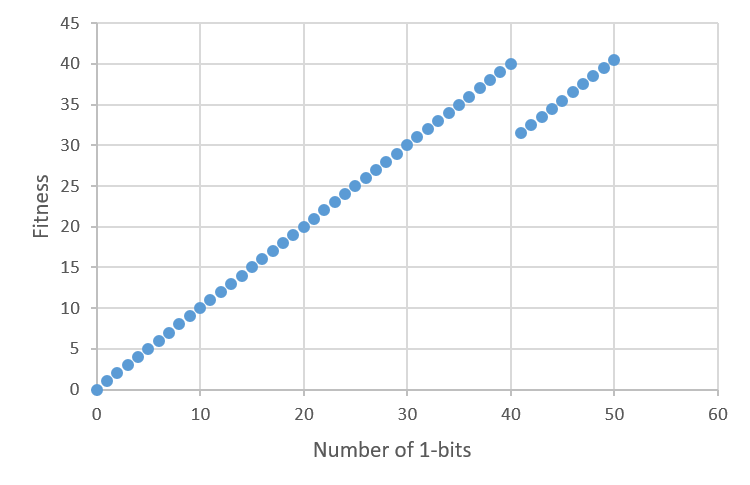
\includegraphics[width=0.5\textwidth]{2}
% \caption{M$_{linHD}$~ vs. $M_{CH}$ on \textsc{OneMax}}
% \label{fig:plot}
% \end{figure}

% \begin{figure}[t!]
% \centering
%  \includegraphics[width=0.5\textwidth]{3}
% \caption{M$_{linHD}$~ for \textsc{LeadingOnes}}
% \label{fig:plot}
% \end{figure}

% \begin{figure}
% \centering
%  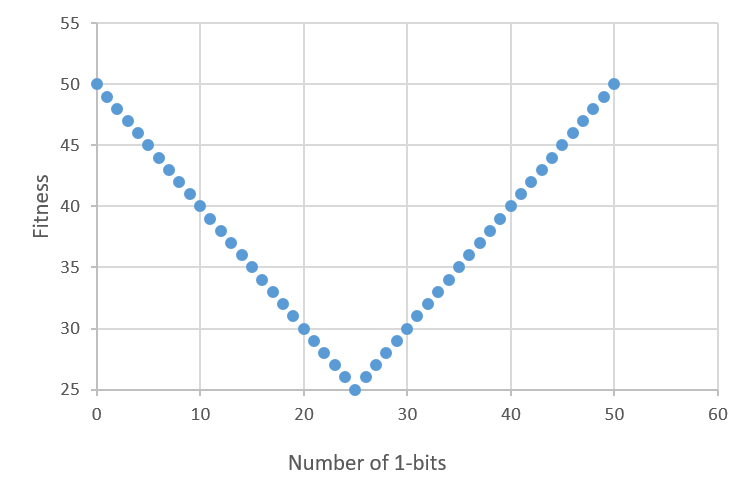
\includegraphics[width=0.5\textwidth]{4}
% \caption{M$_{linHD}$~ for \textsc{LeadingOnes}}
% \label{fig:plot}
% \end{figure}

% \begin{figure}[t!]
% \centering
%  \includegraphics[width=0.5\textwidth]{5}
% \caption{$M_C$ for \textsc{OneMax}}
% \label{fig:plot}
% \end{figure}



%Table \ref{tab:1} shows a summary of the discussed results 
%by (1+1)~IA$^{hyp}$ using inversely proportional hypermutations with different 
%mutation potentials and (1+1)~IA$^{hyp}$ using static hypermutations for 
%optimising \textsc{OneMax} and \textsc{LeadingOnes}.

Given that {\expoHD } provides larger hill-climbing speed-ups compared to the other mutation potentials and is stable to the scaling of fitness functions,
we will use it in the remainder of the paper.

\textcolor{purple}{However, {\expoHD } only allows to flip at most $\sqrt{n}$ bits when far away from the optimum, which means that apart from at initialisation the algorithm hardly ever hypermutates.}

 	
 	\section{Inefficient Behaviour of IPH in Practice}In this section we consider the usage of  {\expoHD } in realistic applications where the optimum is unknown.
 	To this end, the best seen solution will be used by the operator, rather than the unknown optimum. {\color{blue} As a design choice, when the algorithm finds a new solution that is as good as the previous best we update the best seen solution.}
 	We combine \IPHfcm{} using {\expoHD } with hybrid ageing, as in the Opt-IA AIS \cite{CutelloNicosiaPavoneTimmis2007}, and embed it in a $(1+1)$~Opt-IA shown in Algorithm \ref{alg:alg1+ageing}. \new{To use the ageing operator an age, $\alpha(x)$, is assigned to the individual $x$ and is initially set to zero.} After the Hypermutate$(x)$ operator, %, our algorithm  
 	%1) calculates $M:=$ \expoHD, and 2) creates $y$ by flipping at most $M$ distinct bits of $x$ selected uniformly at random one after another until constructive mutation happens.
 	the ageing operator is applied.
 	Among the different variants of ageing, {\it hybrid} ageing has been shown to be very efficient at escaping local optima~\cite{OlivetoSudholt2014ageing,CorusOlivetoYazdaniGECCO2017,CorusOlivetoYazdaniPPSN2018Approx}. Using this operator,  individuals are assigned with initial age zero. During each iteration of the algorithm, the age  increases by 1 and is passed to the offspring if it does not improve over its parent's fitness. If the offspring is fitter than the parent, then its age is set to 0. At the end of each iteration, any individual with age larger than a threshold $\tau$ is removed with probability $1/2$. In case there is no other individual left, a new individual is initialised uniformly at random. 
 
 Ageing has been shown to enable algorithms to escape from local optima either by identifying a gradient leading away from it or by restarting the whole optimisation process. Our aim behind the algorithm design is that by escaping local optima via ageing, the number of local optima that are identified by the algorithm increases over time. Thus as time goes by {\expoHD } should approximate its ideal behaviour better and better.
 	However, we will show that this is not the case. For the purpose we consider the well-studied
 	%In this section we analyse a more realistic version of Algorithm \ref{alg:simple} with mutation potentials that consider the best individual seen so far instead of the optimum. Combined with hybrid ageing to make it capable of escaping difficult local optima, we analyse the resulting algorithm (shown in Algorithm \ref{alg:alg1+ageing}) on 
 	bimodal benchmark function \textsc{TwoMax} % shown in~(\ref{func:twomax}) and 
 	illustrated in Figure~\ref{fig:twomax}~\cite{FriedrichOSWECJ09,SudholtBookChapter2019,OlivetoSudholtZarges2018,CovantesOsunaSudholt2017,CorusLissovoiOlivetoWittTELO2021}:
 	
 	\begin{equation}\label{func:twomax}
 		\textsc{TwoMax}(x):=\max \left\{\sum_{i=1}^n x_i, \; n-\sum_{i=1}^n x_i \right\}.
 	\end{equation} 
 	
 	\textsc{TwoMax} is often used to evaluate the global exploration capabilities of evolutionary algorithms, i.e., whether the population can identify both optima of the function. The standard $(\mu+1)$~EA fails to identify both optima of \textsc{TwoMax} efficiently, hence, the function has been often used to evaluate the effectiveness of diversity mechanisms for improving the global exploration capabilities of populations-based EAs~\cite{FriedrichOSWECJ09,SudholtBookChapter2019,OlivetoSudholtZarges2018,CovantesOsunaSudholt2017}. \new{Recently Corus et al.~\cite{CorusLissovoiOlivetoWittTELO2021} have been shown that artificial diversity mechanisms are not necessary for the $(\mu+1)$~EA to efficiently identify both optima of the function. It suffices to decrease the selection pressure of the algorithm e.g., by employing  inverse tournament selection. In particular, they show that the reason why the traditional $(\mu+1)$~EA fails is that the uniform parent selection usually employed leads to premature convergence of the population.
 	With sufficiently low selective pressure and a linear population size the $(\mu+1)$~EA can optimise  \textsc{TwoMax} in approximately $\Theta(n^2 \log n)$ w.o.p.~\cite{CorusLissovoiOlivetoWittTELO2021}.} In the next section we will present an AIS using IPH that is considerably faster.
 	
 	In this section, our analysis shows that once the $(1+1)$~Opt-IA using \IPHfcm{} with \expoHD{}  escapes from one local optimum, the mutation rate will increase as the algorithm climbs up the other branch.
 	As a result, the algorithm struggles to identify the other optimum and wastes more and more fitness function evaluations as it approaches it. Thus, the whole purpose behind IPH is defeated.
 	
 	On the bright side, we will show that {\expoHD } combined with ageing can efficiently escape from local optima. We will use the well known \cliff{} function %(shown in  (\ref{func:cliff})) 
 	for this purpose where static hypermutations are inefficient:
 	\begin{equation} \label{func:cliff}
 		\textsc{Cliff}_{d}(x):=\begin{cases}
 			\sum_{i=1}^n x_i & \text{if}\; \sum_{i=1}^n x_i \leq n-d, \\
 			\sum_{i=1}^n x_i -d+ 1/2 & \text{otherwise.}
 		\end{cases}
 	\end{equation}
 	The class of \textsc{Cliff} functions, illustrated in Figure~\ref{fig:cliff}, is usually used to assess the performance of non-elitist algorithms. %is another widely used multimodal benchmark function which 
 	It was originally designed as a problem instance where non-elitist EAs outperform elitist EAs~\cite{JaegerskuepperStorch}. This function  has a \textsc{OneMax} slope with length $n-d$ which leads the algorithms towards the local optima. The local optima are followed by a second \textsc{OneMax} slope (of length $d$) of lower fitness which leads to the global optimum. While elitist algorithms need to make a jump of size $d$ to find the global optimum, non-elitist algorithms can easily find the second slope by accepting inferior solutions, %by a mutation size which is as small as 1, then 
 	and then hillclimb up to the global optimum \cite{LissovoiOlivetoWarwicker2019AAAI,CorusOlivetoYazdani2019TCS,CorusOlivetoYazdani2021TEVC,HeviaSudholtAlgo24}. 
 	Due to the high mutation rates of static hypermutations, even if they were to escape the local optima of \textsc{Cliff} (which is unlikely due to FCM and linear mutation potentials), they would still jump back with high probability.  
 	%However,  elitist algorithms can only find the global optimum by making a jump of size $d$ (hence, they will have the same runtime as for \textsc{Jump}). 
 	
 	%The performance of various evolutionary algorithms and diversity preserving mechanims for the global optimisation of $\textsc{TwoMax} $ have been inverstigated in the literature 
 	
 	
 	
 	%\begin{algorithm}[t] 
 	%    \caption{$(1+1)$~Opt-IA with \expoHD}
 	%    \begin{algorithmic}[1] % The number tells where the line numbering should start
 		%             \STATE{Initialise $x \in\{0,1\}^n$ uniformly at random;} %and add to $P$;}
 	%            \STATE{set $\alpha(x):=0$ and $\text{best}:=x$};      
 	%            \STATE evaluate $f(x)$;    
 	%            \WHILE{termination condition is not satisfied} %\Comment{} 
 	%             \STATE{$\alpha(x):=\alpha(x)+1$};
 	%             \STATE{ $M :=$ \expoHD};
 	%            %\STATE{$y \leftarrow invHyp(x)$}
 	%            \STATE{create $y$ by flipping at most $M$ distinct bits of $x$ 
 		%selected uniformly at random one after another until a \textit{constructive 
 			%mutation} happens;}
 	%            \IF{$f(y) > f(x)$}
 	%            \STATE{$\alpha(y):=0$};
 	%            \ELSE
 	%            \STATE{$\alpha(y):=\alpha(x)$};
 	%            \ENDIF
 	%            \IF{ $f(y)\geq f(\text{best})$}
 	%            \STATE{ then set $\text{best}:=y$};
 	%            \ENDIF
 	%            %\STATE{Add $y$ to $P$};
 	%            \FOR{$w \in \{x,y\}$}
 	%			\IF{$\alpha(w) \geq \tau$}
 	%			\STATE{with probability $1/2$, reinitialise $w$ uniformly at random with $\alpha(w)=0$}; 
 	%			%\STATE {Select the best individual in $P$ and remove the other};
 	%			\ENDIF
 	%			\ENDFOR
 	%			\STATE{Set $x=\arg\max\limits_{z\in\{x,y\}}f(z)$; }
 	%			%\STATE{If $|P|=0$, create $x \in\{0,1\}^n$  uniformly at random with $x.age=0$ and add $x$ to $P$;}
 	%            \ENDWHILE
 	%    \end{algorithmic} \label{alg:alg1+ageing}
 	%\end{algorithm}
 	
 	\begin{algorithm}[t] 
 	\caption{$(1+1)$~Opt-IA}
 	\begin{algorithmic}[1] % The number tells where the line numbering should start
 		\STATE{Initialise $x \in\{0,1\}^n$ uniformly at random;} %and add to $P$;}
 	\STATE{set $\alpha(x):=0$ and $\text{best}:=x$};      
 	\STATE evaluate $f(x)$;    
 	\WHILE{termination condition is not satisfied} %\Comment{} 
 	\STATE{$\alpha(x):=\alpha(x)+1$};
 	\STATE{$y:=\text{Hypermutate}(x)$}
 	%             \STATE{ $M :=$ \expoHD};
 	%            %\STATE{$y \leftarrow invHyp(x)$}
 	%            \STATE{create $y$ by flipping at most $M$ distinct bits of $x$ 
 		%selected uniformly at random one after another until a \textit{constructive 
 			%mutation} happens;}
 	\IF{$f(y) > f(x)$}
 	\STATE{$\alpha(y):=0$};
 	\ELSE
 	\STATE{$\alpha(y):=\alpha(x)$};
 	\ENDIF
 	\IF{ $f(y)\geq f(\text{best})$}
 	\STATE{ then set $\text{best}:=y$};
 	\ENDIF
 	%\STATE{Add $y$ to $P$};
 	\FOR{$w \in \{x,y\}$}
 	\IF{$\alpha(w) \geq \tau$}
 	\STATE{with probability  $p_{\text{die}}=1/2$, reinitialise $w$ uniformly at random with $\alpha(w)=0$}; 
 	%\STATE {Select the best individual in $P$ and remove the other};
 	\ENDIF
 	\ENDFOR
 	\STATE{Set $x=\arg\max\limits_{z\in\{x,y\}}f(z)$; }
 	%\STATE{If $|P|=0$, create $x \in\{0,1\}^n$  uniformly at random with $x.age=0$ and add $x$ to $P$;}
 	\ENDWHILE
 	\end{algorithmic} \label{alg:alg1+ageing}
 \end{algorithm}


\begin{figure}
\begin{minipage}{.5\textwidth}
\centering
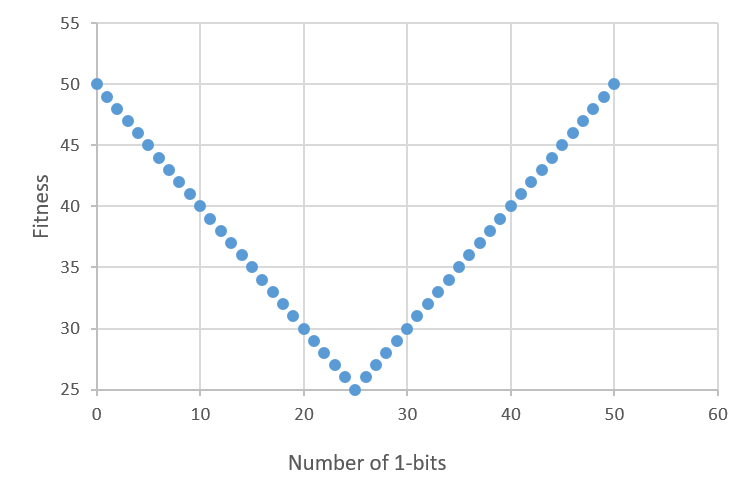
\includegraphics[width=1\textwidth]{4}
\caption{The \textsc{TwoMax} test function for $n=50$}
\label{fig:twomax}
\end{minipage}
\begin{minipage}{.5\textwidth}
\centering
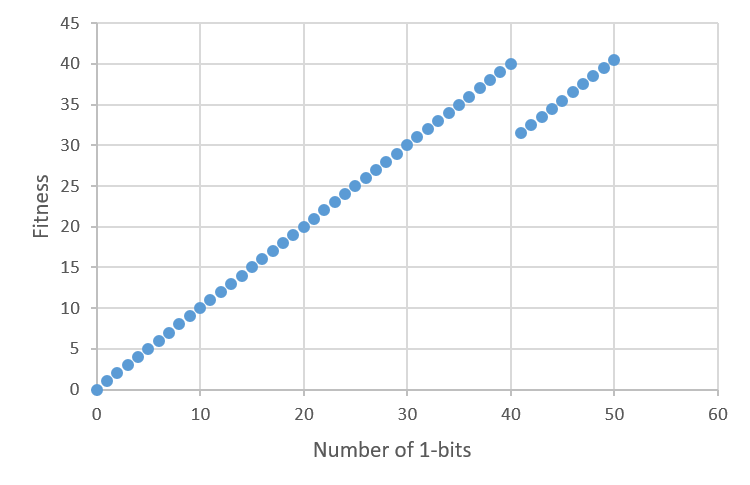
\includegraphics[width=1\textwidth]{2}
\caption{The \textsc{Cliff} test function for $n=50$ and $d=10$}
\label{fig:cliff}
\end{minipage}%
\end{figure}







% 
%  \begin{figure}[t!]
% \centering
%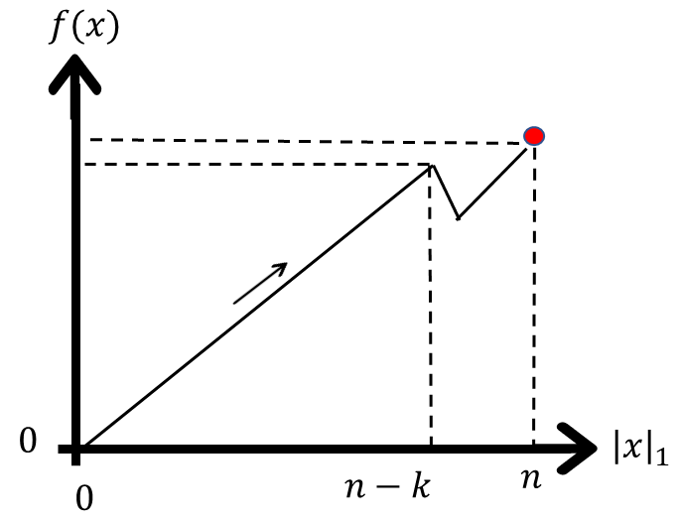
\includegraphics[width=0.2\textwidth]{cf}
%\caption{\textsc{Cliff} test function}
%\label{fig:benchmarks}
% \end{figure}

%\textsc{TwoMax} is often considered in the literature to evaluate the global optimisation capabilities of evolutionary algorithms by verifying whether both optima may be identified by 
%populations.
We start by showing that without knowing the location of the optimum in advance the algorithm becomes very efficient for hill-climbing on \textsc{OneMax} and \textsc{LeadingOnes}.

\begin{theorem} \label{thm:onemaxexpo}
The expected runtime of the \oneoneOPTIA~using \IPHfcm{}  with {\expoHD } for optimising
\textsc{OneMax} is $\Theta(n\log n)$ with $\tau=\Omega(n^{1+\epsilon})$ {\color{blue}for any arbitrary} constant $\epsilon>0$.
\end{theorem}
\begin{proof}
Let $x_t$ be the current solution at the beginning of the iteration $t$. Immediately after the initialisation, the best seen solution is the current individual $x_1$ itself and the mutation potential is $M=$ {\expoHD }$=n^{H(x_1,x_1)/n}=n^0=1$. Note that  $x_t \neq x_{t+1}$ if and only if either $f(x_{t+1})\geq f(x_t)$ or $x_{t+1}$ is reinitialised after $x_t$ is removed from the population due to ageing. Thus, the mutation operator flips a single bit at every iteration until ageing is triggered for the first time.
The improvement probability will be at least $ 1/n $ until either $1^n$ or $0^n$ is sampled. 
Given that the ageing threshold $\tau$  is at least $n^{1+\epsilon}$ for some constant $\epsilon >0 $, 
the probability that the current solution will not improve $\tau$ times consecutively is at most 
$(1-\frac{1}{n})^{n^{1+\epsilon}}=e^{-\Omega(n^\epsilon)}$. 
Hence, the first optimum will be found before ageing is triggered w.o.p. Given that the ageing operator is not triggered, the expected time to find the first optimum can be shown with a fitness level argument. Let $k$ be the number of $0$-bits in $x_t$. The probability that a mutation improves $x_t$ is thus $k/n$ and the expected time for such an improvement is $n/k$. If we sum over all possible $k$, we obtain the expected runtime $\sum\limits_{k=1}^{n}n/k \leq n \ln n + {\color{blue}O(n) } $, which is conditional on ageing not being triggered. If ageing triggers, the mutation potential can be at most $n$ and due to FCM the runtime would be at most $O(n^2 \log n)$ following the same line of argument while considering $n$ wasted fitness function evaluations for each mutation. As the reinitializations are uniformly at random if we pessimistically assume that the first instance of ageing triggering happened at level $n-1$ which yields the maximum mutation potential,  Since the ageing does not trigger with overwhelming probability, the expected runtime is $O(n \log{n})$.

To prove the lower bound we make a case distinction with respect to whether the ageing is triggered before the optimum is found. If the ageing mechanism is triggered, then by our assumption $\tau=\Omega(n^{1+\epsilon})$ the runtime is $\Omega(n \log n)$. For the second case, the operator flips a single bit per mutation. Since the algorithm is initialised with a uniformly random solution, the number of $0$-bits in the initial solution is at least $n/3$ w.o.p. due to Chernoff bound on the binomial distribution. Similar to our argument for the upper bound, the expected time until the number of $0$-bits in the solution decreases from $k$ to $k-1$ is $k/n$. Therefore, the expected runtime is  at least $(1-2^{-\Omega(n)}) \cdot \sum_{k=1}^{n/3} k/n = \Omega(n \log n)$. 
\end{proof}

\begin{theorem} \label{thm:leadingonesexpo}
The expected runtime of the \oneoneOPTIA~using \IPHfcm{}  with {\expoHD } for optimising
\textsc{LeadingOnes} is $\Theta(n^2)$ with $\tau=\Omega(n^{1+\epsilon})$ {\color{blue}for any arbitrary} 
constant $\epsilon>0$.
\end{theorem}
\begin{proof}
For any suboptimal $x\in\{0,1\}^n$ it is sufficient to flip the leftmost $0$-bit of $x$ to improve its \textsc{LeadingOnes} value. Thus, the same argument in Theorem~\ref{thm:onemaxexpo} which establishes that the ageing will not trigger with overwhelming probability also holds. We can similarly continue with a fitness level argument, {\color{blue} with the only difference in that} the improvement probability for \textsc{LeadingOnes} is always $1/n$ regardless of the current function value and thus the sum yields $\sum\limits_{i=1}^{n}n = n^2$.

For the lower bound, it is sufficient to prove that the {\color{blue}expectation conditional on ageing not triggering} is $\Omega(n^2)$, since ageing will not trigger with overwhelming probability. In that case we have to consider how much the objective function value will increase in expectation when the leftmost $0$-bit is flipped by the operator. The bits on the right of the leftmost $0$-bit does not contribute to the fitness value and thus each can be a $0$-bit or $1$-bit with equal probability. Therefore, the expected number of "free-riders", i.e., the sequence of consecutive $1$-bits that follow the leftmost $0$-bit is at most $\sum_{i=0}^{n}2^{-i}\leq 2$. Since the expected increase after every mutation is at most $2$, the expected number of necessary successful mutations where the leftmost $0$-bit is flipped is at least $n/2$ to find the optimal solution. The expected time for each such successful mutation is $(1/n)^{-1}=n$ iterations and consequently the expected time until the optimum is found given that the ageing operator does not trigger is $\Omega(n^2)$.  
\end{proof}
We now move on to \textsc{TwoMax}. The following theorem shows that after the algorithm escapes from the local optimum, the mutation rate increases as the algorithm climbs up the opposite branch.
This behaviour causes a large waste of fitness evaluations defying the objectives of IPH.
\begin{theorem}\label{thm:twomaxexpo}
	The expected runtime of the \oneoneOPTIA{} using \IPHfcm{} with
	the {\expoHD} mutation potential for optimising
	\textsc{TwoMax} is $\Theta(n^{2}\log n + {\color{blue}\tau})$, provided the ageing
	threshold satisfies $\tau=\Omega(n^{1+\epsilon})$  {\color{blue}for any arbitrary} constant
	$\epsilon>0$.
\end{theorem}

\begin{proof}
	We follow the same argument in Theorem~\ref{thm:onemaxexpo} to conclude that in expected $O(n\log n)$ time, the algorithm will find one of the optima. {\color{blue} Without losing generality, let $1^n$ be the first optimum that the algorithm samples}. 
	
	After finding the first optimum, no single-bit flip can yield an equally fit solution. {\color{blue}Thus, after $\tau$ steps ageing will trigger since the current solution cannot improve. After $n$ steps the probability that the old solution has not died is $\left(1-2^{-n}\right)$ }  Thus, with 
	$\left(1-2^{-n}\right) \cdot \left(1-e^{-\Omega(n^\epsilon)} \right)$ probability a new solution will be initialised within $\tau + n$ steps. Now, the current \emph{best seen} is the first discovered optimum until a new optimum is sampled again. 
	
	Let the first and second branch denote the subsets of the solution space which consist of solutions with less than and more than Hamming distance $n/2$ to the first discovered optimum respectively. We first consider the case when the new solution is initialised on the first branch. Given that the current solution has fitness $i$, the distance to the best seen is $n-i$ and the mutation potential is $M=n^{\frac{n-i}{n}}$. Since the first constructive mutation ensures that the probability of improvement is always at least $1/n$, w.o.p.,  ageing will not be triggered until either optimum is discovered. Thus, given that the current solution is always on the first branch, the proof of Theorem~\ref{cor:omexpohd} carries over and the expected time to find the first discovered optimum once again is at most $O(n^{3/2}\log{n})$ in expectation. When the first discovered optimum is sampled again, w.o.p. the current solution is reinitialised with the first discovered optimum as the best seen solution in at most $\tau + n$ iterations.
	
	Now, we consider the case where the current solution is on the second branch. A lower 
	bound on the probability that the current solution will reach the optimum of the second branch before 
	sampling an improving solution on the first branch will conclude the proof since the expected time to do so is $O(n^{3/2}\log{n})$ given that the current solution does not switch branches before. 
	% 
	
	{\color{blue}Let $n/2 + k$ be the number of $0$-bits in a second branch solution. In order to sample a solution with at least $n/2 +k$ $1$-bits, i.e., a solution with at least equal fitness on the other branch, at least $2k$ bits must be flipped. We will first show that for $k \in [ \sqrt{n},n/2-1]$ the mutation potential $M(k)=n^\frac{n/2 -k}{n}$ is always smaller than $2k$. We will analyse the sign of the function 
	
	\begin{align*}
		 n^{\frac{n/2 -k}{n}} < 2k \iff f(k):= \ln{2k} - (1/2 - k/n)\ln{n}  > 0
	\end{align*}
	
	We will first consider the endpoints of the interval.
	For large enough $n$, $f(\sqrt{n})=\ln{2}-\frac{\ln{n}}{\sqrt{n}}$ and  $f(n/2 -1 )=\frac{\ln{n}}{n} - \ln{(n-2)}$ are both positive. The first derivative of $f(k)$ is $f'(k)=\frac{1}{k} - \frac{\ln{n}}{n}$ whose critical point $k=\frac{n}{\ln{n}}$ lies in the interval $[\sqrt{n},n/2-1]$. In particular, $f$ increases on $[\sqrt{n}, n/ \ln{n}]$ and decreases on $[n/\ln{n},n/2 -1 ]$, concluding that it stays positive for the entire interval. Consequently, we have established that once the individual on the second branch has at least $n/2 + \sqrt{n}$ $0$-bits, the hypermutation operator can not yield an equally good solution on the first branch. 
	
	Next, we will argue that a reinitialised solution has a $\Omega(1)$ probability of having at least $n/2 + \sqrt{n}$ $0$-bits. Since the number of $0$-bits is $Bin(n, 1/2)$ distributed, the desired event is that the outcome deviates at least by two standard deviations from the mean and has probability $1-\phi(2) = \Omega(1)$. 
	
}

	 Given that no switch occurs, the expected time to find the second optimum is $\sum_{i=1}^{n/2+\epsilon n} \frac{n}{i} \cdot 
	n^{\frac{n-i}{n}}=O(n^{2}\log{n})$. Since, we will have to restart a constant number of times in expectation until we guarantee that the solution will not switch until the second optimum is found, the expected time to find both optima is $O(n^{2}\log{n})$.
	
	For the lower bound, assume that the first discovered solution is $1^n$ and consider the last $\frac{n}{\log{n}}$ fitness-levels before the second optimum $0^n$ is discovered. Due to FCM, the current solution has to visit each of these levels and the minimum mutation potential in these fitness levels is $n^{\frac{n-n/\log{n}}{n}}=\frac{n}{e}$. Thus, the expected time is at least $\sum_{i=1}^{n/\log{n}} \frac{n}{i}\cdot \frac{n}{e} = \Omega(n^2 \log{n})$. 
	
	
	
\end{proof}


%\begin{theorem}
%The expected runtime of Algorithm \ref{alg:alg1+ageing} with \expoF to optimise \textsc{TwoMax} is $?$ with $\tau=?$.
%\end{theorem}


%\begin{theorem}
%The expected runtime of Algorithm \ref{alg:alg1+ageing} with \expoHD to optimise \textsc{TwoMax} is $?$ with $\tau=?$.
%\end{theorem}

%\begin{equation*}
%\textsc{Cliff}_{d}(x)=\begin{cases}
%		\textsc{OneMax}(x) & \text{if}\; \textsc{OneMax}(x) \leq n-d \\
%        \textsc{OneMax}(x)-d+ 1/2 & \text{otherwise}
% \end{cases}
%\end{equation*}


%\begin{theorem}
%Algorithm \ref{alg:alg1+ageing} with \linHD cannot optimises \textsc{Cliff}$_k$. {\color{red} not completed}
%\end{theorem}

%\begin{proof}
%W.o.p the initialised solution has at least $n/2-\epsilon n$ 0-bits. At the beginning, we assume the smallest $M$ is 1 again. Hence it has the same behaviour as RLS and finds the local optimum (i.e., edge of the cliff) in $\Omega(n \log n)$. Then the individual will reach age $\tau$ and die with probability $1/2$. At the same iteration that it dies, an individual will be created down the cliff with age $\tau$ and stays alive with probability 1/2. The best seen is now the local optimum. Hence, the mutation potential increases at each step towards the optimum. At the button of the cliff, $M=1$. With probability $(n-k)/n$ the individual will go back and with probability $(k-1)/n$ it will go up. If it doesn't go back, at the next step with probability $(k-2)/n$ it will follow the direction towards the optimum, and with probability $(n-k+1)/n$. Looking at the last step, the probability of going back is at least $(\frac{n-1}{n})^2$. Seems like the same case as TwoMax.
% 
%\end{proof}

%\begin{theorem}
%Algorithm \ref{alg:alg1+ageing} with \expoF on  \textsc{Cliff}$_k$. 
%\end{theorem}

%\begin{proof}
%After initialisation, as the best seen is the individual itself, $M$ is 1. Hence, the algorithm again behaves like RLS and would find the local optimum in $O(n \log n)$. With probability $k/n$ an offspring would be created  down the cliff at the same iteration that the parent dies. And there is an increasing probability of going back,but maybe is small. In the last step, the probability of finding the optimum is $1/n$ while the probability of going back is almost 1.
%\end{proof}
%
%\begin{theorem}
%Algorithm \ref{alg:alg1+ageing} with \expoHD on  \textsc{Cliff}$_k$. 
%\end{theorem}
%\begin{proof}
%After initialisation, as the best seen is the individual itself, $M$ is 1. After reaching the local optima in $O(n \log n)$, it will die with probability $1/2$ and at the same time an individual is created down the cliff. knowing that the best seen is now the edge of the cliff, $M=n^{1/n}$, which is close to 1 for large $n$. 
%\end{proof}

%\begin{theorem}
%Algorithm \ref{alg:alg1+ageing} with \linHD cannot optimise \textsc{LeadingOnes-LeadingZeroes}.
%\end{theorem}

%\begin{proof}
%Without lose of generality we assume the initialised bit string is on the \textsc{ZeroMax} slope. At the beginning, $M=1$ and hence the algorithm has the same behaviour as RLS. With probability at least $1/n$ the individual will improve towards the $0^n$. As $M=1$, the probability of jumping to the other branch after fitness level $i=2$ is zero. The individual will follow the branch towards $0^n$ and in $O(n^2)$ it will reach the $0^n$. Then the individual will die with probability 1/2 as it cannot reach $1^n$. Being reinitialised (the prob that we don't start in the left branch again? and how many times we might restart from the same branch), now the best seen is $0^n$.   Same as before, the individual will progress toward $1^n$ with probability at least $1/n$. Showing the number of leading 1-bits with $i$, the probability of jumping to the other branch (the same fitness) is at least  $n^{-(i+1)}$. At the last step, $M=n$, so it is very probable that we jump to the other branch. The probability that we reach $1^n$ from $1^{n-1}0$ is $1/n$ and the probability of jumping to other branch is at least $(n-1)/n$. 
%%Conditional probability on the first event happening before the second is very close to 1. Hence the total expected runtime would be $O(n^2)+ cn^2+\sum_{i=1}^{n} n \cdot (n-i)$
%\end{proof}

%\begin{theorem}
%Algorithm \ref{alg:alg1+ageing} with \expoF on \textsc{LeadingOnes-LeadingZeroes}. 
%\end{theorem}
% 
% \begin{theorem}
% Algorithm \ref{alg:alg1+ageing} with \expoHD on  \textsc{LoLz}. 
% \end{theorem}
Now we show that differently from static hypermutations, {\expoHD }
combined with ageing can escape from the local optima of \cliff, 
hence optimises the function efficiently. The condition that $d$ is not prohibitively large is necessary to avoid
that the reinitialised solutions due to ageing have larger fitness than a solution with $n-d+1$ $1$-bits, {\color{blue} which would cause the latter to be removed from the population}.
We believe that this assumption is realistic for practical applications.

\begin{theorem}\label{thm:cliffexpo}
The {\oneoneOPTIA } using \IPHfcm{} with {\expoHD } and $\tau=\Omega(n^{1+\epsilon})$ 
for 
an arbitrarily small constant $\epsilon$,  optimises \cliff{} with 
$d<n(\frac{1}{4}-\epsilon)$ in expected {\color{blue} $O\left( \left(n^{3/2}\log{\frac{n}{d}}+\tau \right)\cdot \frac{n^2}{d^2}\right)$ }
 fitness function evaluations. 
\end{theorem}

\begin{proof}
The analysis will follow a similar idea to the proof of 
Theorem~\ref{thm:twomaxexpo}. After initialisation, the initial mutation 
potential is $M=1$ since the current solution is the best seen solution. With 
single bit-flips it takes in expectation at most {\color{blue}$O(n \log{\frac{n}{d}})$} to find 
a local optimum of the cliff (i.e., a search point with $n-d$ 1-bits). Since the 
local optima {\color{blue} have better fitness value than any other suboptimal solution, as long as the current solution is a local optimum, $M=1$ regardless of how many restarts happened before. Moreover,} a local optimum cannot be improved with single bit flips and in $\tau$ generations after it was first discovered the ageing will be triggered and in the following 
$n$ steps the current solution will be removed from the population due to 
ageing with probability at least {\color{blue} $1-\frac{4}{3}^{-n}$}. The Hamming distance of the  
reinitialised solution will be distributed binomially with parameters $n$ and 
$1/2$ and w.o.p. will be smaller than $n/2 + 
n^{2/3}$, yielding an initial mutation potential of $M{\color{blue}\leq n^{\frac{n/2+n^{2/3}}{n}}=n^{1/2}\cdot n^{n^{-1/3}}=} O(n^{1/2})$. {\color{blue}Since we only consider improvements after the first bit-flip,} we 
pessimistically assume that the mutation potential will not decrease until a  
local optima is found again, which implies that the expected time {\color{blue} between the consecutive discoveries of the local optima} will be at 
most {\color{blue}$O(n^{3/2}\log{\frac{n}{d}}+\tau)$ } since each iteration will waste an extra 
$O(n^{1/2})$ fitness function evaluations {\color{blue} until finding a local optimum}. After finding a local optimum 
again, the mutation potential will be $M=1$ since it will replace the 
previously observed local optimum as the best seen. The process of 
reinitialisation and reaching the local optima will repeat until a solution at the bottom of the Cliff is created and accepted.

If the local optima produces an offspring with $n-d+1$ bits, which happens  with probability 
$d/n$ and if this solution survives the ageing operator (with 
probability $(1-p_{\text{die}})$), then  the reinitialised solution will be rejected w.o.p. 
since its fitness value will be smaller than $n-d$ due to our assumption $d<n(\frac{1}{4}-\epsilon)$. 
The Hamming distance of this new solution to the best seen will be exactly one 
since it is created via a single bit-flip, thus its mutation potential 
will be $M=1$.  Moreover, if the surviving offspring improves again (with 
probability $(d-1)/n$) in the next iteration, it will reset its age to zero and 
will 
have Hamming distance of at least two to any local optima.  In expected 
$O(n\log d)$ generations, this solution will reach 
the global optimum unless a solution with less or equal $n-d$ 1-bits is sampled 
before. {\color{blue}While $M=1$, the distance to the local optima can only increase by improvements. In particular until we have improved for $\ln{2}\cdot n / \ln(n)$ times, which gives us the minimum distance to the local optima which yields $M\geq 2$. The distance of any individual on the second slope to any local optimum is bounded by $2d<n/2$ which implies that $M\leq \sqrt{n}$ and also that we will never be able to sample a solution with at most $n-d$ 1-bits since all bitstrings with $M>1$ have more than $\sqrt{n}$ distance to the local optima. }  Therefore, 
once a solution with $n-d+2$ bits is added to the population, the algorithm 
finds 
the optimum in {\color{blue}$O(n\log{d})$} iterations and in at 
most {\color{blue} $O(n^{3/2}\log{d})$} fitness function evaluations since the mutation 
potential is at most $\sqrt{n}$. The probability of obtaining a solution with 
$n-d+2$ 1-bits at the end of each cycle of reinitialisation and removal of the 
local optima due to ageing  is $(1-p_{\text{die}})^2 \cdot (d/n)\cdot ((d-1)/n)$. Since each such cycle 
takes {\color{blue}$O(n^{3/2}\log{\frac{n}{d}}+\tau )$} fitness evaluations, our claim follows after absorbing smaller order term into $O\left(\left(n^{3/2}\log{\frac{n}{d}}+\tau\right)\cdot \frac{n^2}{d^2} \right)$.
% use the Ballot Theorem to bound the Hamming 
% distance given the number of 1-bits. Ballot theorem implies that sampling an 
% solution at least as good as the parent (which are the only solutions that are 
% accepted) has probability at most $2 i /n$ where $i$ is the number of 0-bits in 
% the solution. Since the probability of improving in the first step is at least 
% $i/n$, we can conclude that the conditional probability that an accepted 
% offspring is a Hamming neighbour of its parent is at least $1/2$ .
\end{proof}

%{\color{red} This also cannot optimise Jump. We can mention this here maybe? Even with ageing.}

\section{An Efficient IPH with Mutation Potentials for Opt-IA} \label{sec:FCMsymmetric}
In the previous section, we observed that towards the end of the optimisation process the mutation potential may increase as the current solution approaches an undiscovered, potentially promising optimum. This behaviour is against the design intentions of the inversely proportional hypermutation operator since in the final part of the optimisation process it gets harder to find improvements and high mutation potentials lead to many wasted fitness function evaluations.
The underlying reason of this behaviour in both the \textsc{Cliff} and \textsc{TwoMax} landscapes is the necessity to follow a gradient that leads away from the local optimum to find the global one. Considering that this necessity would be ubiquitous in optimisation problems, we propose a new method to control mutation potentials in this section. The newly proposed mutation potential is called {\it Symmetric \expoHD} and is defined as:
%\begin{equation}
%\text{Symmetric M}_{\text{expoHD}}:= \left\lceil n \cdot 
%n^{-\frac{HD(x,x.org)}{\max\{HD(best,x.org), 1\}}} \right\rceil.
%\end{equation}
\begin{equation} \label{eq:symexpoHD}
\text{Symmetric M}_{\text{expoHD}}:= \max \left\{\left\lfloor  
n^{\frac{H(\text{best},\text{org}(x))-H(x,\text{org}(x))}{n}} \right\rfloor , 1\right\}.
\end{equation}

Symmetric \expoHD{} uses a mutation potential that is inversely proportional to the current solution's Hamming distance to its origin, where the origin (returned by org$(x)$ in (\ref{eq:symexpoHD})) is defined as the ancestor of the current bit string after the last removal of a solution due to ageing (Figure~\ref{fig:symexpoHD}) i.e., the re-initialised individual or the one that survived ageing.  At initialisation, the origin of each solution is set to itself and the newly created offspring inherit the origin of their parents. 


This mutation potential reliably decreases (at the same rate it would decrease if it was approaching the currently best seen local optimum) as the current solution improves and moves away from its origin up until it starts doing local search and finds a local optimum. Every time a local optimum is found, ageing is triggered after approximately $\tau$ steps and then both surviving and reinitialised individuals reset their origin to their own bit string. We   embed \IPHfcm{} with Symmetric \expoHD{} in Algorithm~\ref{alg:symmetric}. %For the function Hypermutation$(x)$, our algorithm performs two steps, 1) it computes $M$ using (\ref{eq:symexpoHD}), then 2) creates $y$ by flipping at most $M$  distinct bits of $x$ selected uniformly at random one after another until a constructive mutation happens.


\begin{figure}[t!]
\centering
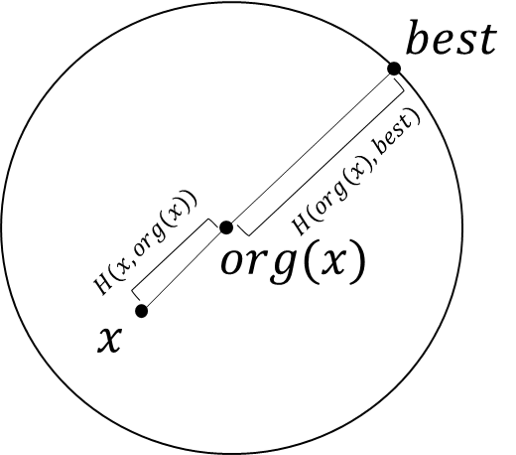
\includegraphics[width=0.3\textwidth]{newhd}
\caption{The geometric representation of Symmetric \expoHD. The mutation potential is determined according to the 
	ratio of the Hamming distance between the current solution ($x$) and its origin ($\text{org}(x)$) and 
	the Hamming distance between its origin and the best seen solution (best).}
\label{fig:symexpoHD}
\end{figure}





%\subsection{The performance of Algorithm~\ref{alg:simple} when the Best found 
%solution is used instead of the optimum}

%\begin{itemize}
% \item When the population size is one, the algorithm uses the minimum mutation 
%potential throughout the run.
%\item Since the hypermutation operator does no allow copies, it is not clear 
%how the mutation potential behaves within a population. However, if the Hamming 
%neighbourhood of the best solution has better fitness than the rest of the 
%population, it is expected that in at most $O(\mu)$ generations the population 
%consists only of individuals with HD one to the best which implies that the 
%higher mutation potential are rarely observed.
%\item We do not know what happens when the characteristic ``no genotype 
%duplicate'' principle of Opt-IA is used.
%\end{itemize}




\begin{algorithm}[t!] 
\caption{(1+1) Opt-IA with symmetric IPH}
\label{alg:symmetric}
\begin{algorithmic}[1] % The number tells where the line numbering should 
	% start
	%\STATE{Set $x \sim Unif(\{0,1\}^n)$ }
	\STATE{Initialise $x \in\{0,1\}^n$ uniformly at random;}
	\STATE {set org$(x):=x$, $\alpha(x):=0$, and best$:= x$;}
	%             \STATE {Set $x.age:=0$;    }
	\STATE {evaluate $f(x)$;   } 
	\WHILE{termination condition not satisfied} %\Comment{}      
	\STATE{$\alpha(x):=\alpha(x)+1$};
	\STATE{$y:=\text{Hypermutate}(x)$ with Symmetric \expoHD{} };
	%            \STATE{$M:=$ Symmetric $M_{expoHD}$;}
	%            \STATE{Create $y$ by flipping at most $M$  distinct bits of $x$ selected uniformly at random one after 
		%another until a \textit{constructive mutation} happens;} 
	\STATE{org$(y):=\text{org}(x)$};
	\IF{$f(y)> f(x)$}
	\STATE{$\alpha(y):=0$};
	\IF{$f(y)\geq best$}
	\STATE {best$:=y$;}
	\ENDIF
	\ELSE
	\STATE{$\alpha(y):=\alpha(x)$};
	\ENDIF
	\FOR{$w \in \{x,y\}$}
	%\IF { $w.age \geq \tau \wedge p_{die}=1/2>R \sim Unif(0,1)$}
	\IF{$\alpha(w) \geq \tau$}
	\STATE{with probability $1/2$, reinitialise $w$ uniformly at random with $\alpha(w)=0$}; 
	%\STATE{Set $w \sim Unif(\{0,1\}^n)$ , $w.age=0$, 	}
	% 			\STATE{Set $w.age=0$; }
	\STATE{set org$(w)=w$}
	% 			\STATE{Set ;}
	\ENDIF
	\ENDFOR
	% 			\IF { $y.age > \tau \wedge p_{die}=1/2>R \sim 
		% Unif(0,1)$}
	% 			\STATE{Set $y \sim Unif(\{0,1\}^n)$ 		}
	% 			\STATE{Set $y.age=0$; }
	% 			\STATE{Set $y.origin=y$;}
	% 			\STATE{Set $x.origin=x$;}
	% 			\ENDIF
	\STATE{Set $x=\arg\max\limits_{z\in\{x,y\}}f(z)$; }
	\ENDWHILE
\end{algorithmic}
\end{algorithm}
Since our results for \textsc{OneMax} and \textsc{LeadingOnes} in the previous section rely on ageing not being triggered, they carry over to the symmetric variant. 
The following theorem shows that once one optimum of \textsc{TwoMax} has been identified, the value of the Symmetric {\expoHD } potential decreases as both optima are approached as desired and the speed-up in the runtime is achieved.

\begin{theorem} \label{th:MexpoTwoMax}
The {\oneoneOPTIA } using \IPHfcm{} with Symmetric {\expoHD } with $\tau=\Omega(n^{1+\epsilon})$ for any 
arbitrarily small constant $\epsilon>0$, needs
$O(n^{3/2}\log{n} + {\color{blue}\tau})$ fitness function evaluations in expectation to optimise \textsc{TwoMax}.
\end{theorem}
\begin{proof}
The expected time until the first branch is optimised is $O(n\log{n})$ 
since the best seen search point is the current best individual and 
consequently the mutation potential is $M=1$. Since the improvement 
probability is at least $1/n$ and $\tau=\Omega(n^{1+\epsilon})$, the ageing 
operator does not trigger before finding one of the optima w.o.p. Once one of the optima is found, ageing reinitialises the 
individual while the first discovered optima stays as the current best seen 
search point. For the randomly reinitialised solution, the Hamming distance to 
the best seen is binomially distributed with parameters $n$ and $1/2$. Using 
Chernoff bounds, we can bound the distance to the previously seen 
optima by at most $n/2 + n^{2/3}$ w.o.p. This 
Hamming distance implies an initial mutation potential of $M< 
n^{\frac{\frac{n}{2}+n^{2/3}}{n}}=n^{\frac{1}{2}+\frac{1}{n^{1/3}}}$ which 
decreases as the individual increases its distance to the origin and can never 
go above its initial value where the distance is zero. {\color{blue} Following a similar argument as in Theorem~\ref{thm:twomaxexpo} with a larger deviation, with constant probability the newly sampled solution will have at least $n/2 + 3\sqrt{n}/2$ $0$-bits since $1-\phi(3) = O(1)$. This implies that the mutation potential will never be large enough to sample a solution in the opposite branch.}
Pessimistically assuming that the mutation potential will be 
$n^{\frac{1}{2}+\frac{1}{n^{1/3}}}=O(n^{1/2})$ throughout the run, we can obtain 
the above upper bound by summing over all levels and using coupon collector's 
argument \cite{OlivetoBookChapter}.
% (\textbf{Note:} Once the middle of the branch is reached the HD to the 
% origin might not be the same as the fitness difference with the origin, however 
% $HD(x,y)$ will always be as large as $|TwoMax(x)-TwoMax(y)|$ as long as $x$ and 
% $y$ are one the same branch. This issue becomes a real problem when a lower 
% bound is sought.)
\end{proof}

Since the Opt-IA using static hypermutations requires $\Theta( n^2 \log n)$ expected function evaluations
to climb up either branch of \twomax{}  \cite{CorusOlivetoYazdani2019TCS}, this result represents a $\sqrt{n}$ speed-up
over static mutation potentials and over the known upper bounds for population based EAs to find both optima w.o.p.
%{\color{red}(do we have any proven result for this?)}.




The following theorem shows that Symmetric {\expoHD } is also efficient for \cliff.
\begin{theorem} \label{th:expoHD-cliff}
The {\oneoneOPTIA } using \IPHfcm{} with Symmetric {\expoHD } and $\tau=\Omega(n^{1+\epsilon})$ optimises \cliff{} with 
$d<n(\frac{1}{4}-\epsilon)$ in 
 {\color{blue} $O\left( \left(n^{3/2}\log{\frac{n}{d}}+\tau \right)\cdot \frac{n^2}{d^2}\right)$ } expected fitness function evaluations.
\end{theorem} 

\begin{proof}
The proof is almost identical to the proof of 
Theorem~\ref{thm:cliffexpo}. The most important distinction is that once a 
solution with $n-d+2$ 1-bits is created, its mutation potential remains as $M=1$ until the global optimum is found. The reason is that when ageing is triggered, the surviving 
solutions all reset their origin to themselves, i.e., start 
doing randomised local search. 

% 
% 
% Initialising from a bitstring with $n/2-\epsilon n$ w.o.p. the mutation 
% potential is initially $M=1$ until the edge of the cliff is found for the first 
% time. At the first step $M=n$ but it drops to 1 at the second step and 
% stays like that until the individual reaches the edge of the cliff as the best seen is the individual itself. As long as $M=1$ the behaviour is similar to (1+1)~RLS$_1$, hence in $O(n \log 
% n)$ the algorithm will find the edge of the cliff and the ageing would not get triggered w.o.p. After reaching the edge, 
% since the fitness cannot be improved, the individual reaches the age $\tau$ and dies with probability $1/2$. 
% At the same iteration, an offspring is created down the cliff with probability $k/n$. With probability $(k-1)/n$ this offspring will improve the towards the optimum and hence it will survive. While moving towards the optimum, the best seen stays as the local optimum. As the Hamming distance of the best and origin does not change while the Hamming distance of the current position and the origin is increasing, hence the mutation potential decreases more and more (not sure what is the maximum one). Hence, in $O(n^{3/2} \log n)$ the optimum will be found. The total expected time will be $O(n \log n)+ \tau+ \left( n^{3/2+\epsilon} \cdot n/k \cdot n/(k+1) \right)=O(\frac{n^{7/2}\log n}{k^2})$.
\end{proof}

{\color{blue}

\section{A Function Class Where IPH is Essential} 
In this section we introduce a function class where inversely proportional hypermutations are essential.
The function class is inspired from one previously used to show the advantages and disadvantages of using high mutation rates in the context of rank-based mutation in population based algorithms~\cite{OlivetoLehreNeumann09}.
In rank-based mutation algorithms~\cite{RankBasedMutation} each individual has a different mutation rate based on their rank in the population i.e., the best individual has a low mutation rate while the worst individual a very high one.
The \textsc{LeadingTrapJump} function was introduced as an example where the use of high mutation rates is detrimental while low mutation rates are efficient. We have slightly modified the location of the trap compared to~\cite{OlivetoLehreNeumann09} for our objectives.
\[
\textsc{LeadingTrapJump}  =
\]
\[
\begin{cases}
0 & \text{if } x = 1^{(9/10)n}* \\
\textsc{LO}(x_i | i>2k+1) + 2k+1 & \text{if } x = 0^{2k+1}1^{(9/10)n - 2k-1}*, \\
n-1 & \text{if } x = 0^{\log n}  \text{(this was n/10)}\\
\textsc{LO}(x) & \text{otherwise}.
\end{cases}
\]
\[
\textsc{LeadingTrapJump2}  =
\]
\[
\begin{cases}
	0 & \text{if } x = 1^{(9/10)n}* \\
	\textsc{LO}(x_i | i>2k+1) + 2k+1 & \text{if } x = 0^{2k+1}1^{(9/10)n - 2k-1}*, \\
	n-1 & \text{if } x = 0^{\log n}y \text{ and } |y|_1>\frac{3n}{4} \\
	\textsc{LO}(x) & \text{otherwise}.
\end{cases}
\]



 Essentially the function consists of a  main \leadingones~ slope of increasing fitness until $(9/10)n -1$ leading ones are reached. From there it is necessary to add a constant number $2k$ of leading zeroes before the last $n/10$ leading ones can be inserted to reach the optimum. However, there is a trap consisting of many leading zeroes ($\log n$ ?) that has fitness value higher than any point other than the optimum. High mutation rates are likely to end up in the trap, while low mutation rates are likely to find the optimum. Naturally  if the values of the local and global optima are switched, then high mutation rates will be successful with high probability, while low mutation rates will fail. In the following we will show that the (1+1) Opt-IA with symmetric IPH efficiently optimises the function independent of the location of the optimum, while SBM will get trapped on the all-ones bit-string with high probability if the trap is globally optimal while static hypermutations with mutation potential get stuck in the trap with high probability when the all-ones bit string is optimal.
 %
 %
 \begin{theorem}\label{th:linHD-LeadingTrapJump}
 The {\oneoneIA } using \IPHfcm{} with {\linHD } optimises \textsc{LeadingTrapJump} 
 \end{theorem}
 \begin{proof}
 
 
 The probability of improvement until $1^{9n/10}*$ is at least $1/n$, i.e., the probability of flipping the leftmost $0$-bit in the first bit-flip. Thus, pessimistically assuming that we flip $n$ bits in every iteration in expected $O(n^3)$ fitness function evaluations we reach the local optimum with $(9n/10)-1$ leading ones. Now, as we won't be able to change the reference on this level we will increase our distance to the initial individual on the level whenever one of the $n/10$ bits in the tail is flipped as the first bit since an equally fit solution is created. in $O(n)$ time to $n/20$ (half of the tail). This will then give us a $n/20$ mutation potential. To be mutated into a $0^{2k+1}1^{(9/10)n-2k-1}*$ solution the parent needs to have its first $2k+1$ bits flipped consecutively which happens with probability $\Omega(n^{2k+1})$ since $k<<n$. On the other hand the probability to mutate a bitstring of the form $0^{\log n}y$ with $|y|_1>3n/4$ solution requires all $\log n$ leading $0$-bits to be flipped and since the mutation potential is $n/20$ the resulting string will satisfy the requirements on the number of $1$-bits as the parent initially have $9n/10$ leading ones. Since $\log n<< n$ the probability of each leading $0$-bit to be picked is $1/20$ and with probability $(1/20)^{\log n} = n ^{1/\log[20]2}> n^{-4.5}$
	 	
	 If the algorithm fails to do either of these mutations in $\tau + n$ iteration then the current solution dies w.o.p. and a new solution is reinitialised. Following the leading ones gradient it will reach another local optima with expected distance at least $n/20$ to the previously seen local optimum whether that local optimum is  (more in the iterations after the $0^{\log n}$ optimum is found first), which allows another $\tau$ iterations to do the jumps. Thus in every $n^3+\tau$ steps we will have at least $\tau$ chances to do the jump. In expectation we will require at most $O(n^{4.5} + n^{2k+1})$ such trial to do both. So in $O\left(\left(n^{5.5} + n^{2k+2}\right) \frac{n^3+\tau}{\tau}\right)$ expected fitness function evaluations both types of optimum will be discovered.
	 

 	

\end{proof} 

	 	-Updating when we restart due to ageing would not be as intuitive when we have a population. We can word it like, "when the best individual in the population dies due to ageing it becomes the new reference."
	 	
	 	The mutation potential will increase as we spend time in a fitness level during the first climb because at every generation there is a constant probability of flipping one of the non-contributing bits and get an equally good solution with hamming distance possibly increased. Possibly we say because over multiple generation a non-contributing bit flip might happen in the same position bringing the hamming distance down by 1. 
	 	The first run will take $\Omega(n^3)$ as well. 


		-Do we regularly fall into the trap: After we sample the first trap point, The argument we need:
		1)A trap local optimum has at least 3n/4 bits
		2)hypermutation cannot convert a string with less than 2n/3 1-bits to one with more than 3n/4 bits 
		3)any bitstring with more than 2n/3 bits can have an hamming distance of at most X to the previously seen local optima which yields a maximum of M(x) potential
		4)With M(x) potential the probability of flipping all log n 0s is at most $n^{f(M(x))}$ which does not happen with constant probability until the leadingones bits are gathered 

}

We will introduce a new parameter $c\leq 1$ for determining our mutation potential when it grows linearly with the Hamming distance since we might prefer to avoid the jump back to previously seen local optimum which will hinder exploration that is the main goal of the high mutation rates.

\linHD $=\min\left(\lfloor c \cdot H(x,\text{best}) \rfloor, 1 \right)$ 

%\begin{theorem} \label{th:expoHD-cliff}
%	The {\oneoneOPTIA } using \IPHfcm{} with \linHD,  $\tau=\Omega(n^{1+\epsilon})$ and $c<1-\epsilon$ optimises \cliff{} with 
%	$d<n(\frac{1}{4}-\epsilon)$ in 
%	{\color{blue}  expected fitness function evaluations.}
%\end{theorem} 
%\begin{theorem}\label{th:expoHD-cliff}
%	The {\oneoneOPTIA} using \IPHfcm{} with \linHD\ (factor $c<\tfrac{2}{3}$), ageing parameter $\tau=\Omega(n^{1+\epsilon})$, optimises \cliff{} with $d<n(\tfrac{1}{4}-\epsilon)$ in expected polynomially many fitness evaluations.
%\end{theorem}
%\begin{proof}
%For a solution initialised uniformly at random, the expected number of iterations until the current solution has exactly $n - d$ one-bits is at most $\sum_{i=d}^{n}\frac{n}{i} = O(\log \frac{n}{d})$. The only solution with better fitness is the $1^n$ bit-string. Thus, ageing will trigger unless the global optimum is found within $\tau$ iterations. We now bound the probability that the current individual with $n - d$ one-bits dies in the same iteration in which hypermutation creates either an equally fit individual or an individual with more one-bits.
%
%If the mutation potential is $M = 1$, the probability of creating a solution with more one-bits is at least $d/n$. This is because it is sufficient to flip one of the zero-bits. If $M > 2$, we consider the probability of creating an equally fit solution. This is possible by first flipping a one-bit into a zero-bit and then flipping a zero-bit into a one-bit. Such an event occurs with probability at least $\frac{d}{n}\cdot \frac{n - d}{n - 1}$.
%
%With probability $1/4$, the parent dies and the offspring survives for another iteration. Since the solution with the best fitness has just died due to ageing, the reference point for the mutation potential is this individual. The surviving individual differs from its parent in at most two bits, and since $c < 1$, the mutation potential is $M = 1$.
%
%We pessimistically assume that the current individual still has $n - d$ one-bits. We bound the probability that in the next iteration it flips a zero-bit into a one-bit (with probability $d/n$), dies, and has its offspring survive (again with probability $1/4$). Thus, given that the current solution has age $\tau$ and $n - d$ one-bits, in at most two iterations we obtain an individual with $n - d + 1$ one-bits. This occurs with probability at least
%\[
%\frac{d^2\cdot(n - d)}{8n^2(n - 1)} = \Omega\left(\frac{d^2}{n^2}\right).
%\]
%
%Again, we focus on the iteration immediately following the one in which such a solution is obtained. We bound the probability that hypermutation increases the number of one-bits by $d/n$. This is because flipping a zero-bit on the first attempt now improves fitness, terminates hypermutation due to FCM, and resets the offspring's age.
%
%From this point onwards we have an individual with Hamming distance at most 3 to the reference
%
%\end{proof}

\begin{lemma}[Canonical start from an ageing cliff-top]\label{lem:can-start-omega-d3}
	Assume the process is at the cliff-top (zero-count $d$) when ageing is triggered, under \IPHfcm{} with mutation potential $M(x)=\max\{1,\lfloor c\,\HD(x,x^\top)\rfloor\}$ for some $c\in(0,1)$, the reference-update rule (“update when a strictly better solution is sampled or a best-fitness solution dies”), and the convention that \emph{ageing resets only on strict improvement}. Then, within at most three iterations, the process reaches the canonical second-slope start
	\[
	r_0=2\qquad\text{and}\qquad \HD(r_0)=2
	\]
	with probability at least $\displaystyle \frac{3}{256}\,\bigl(\tfrac{d}{n}\bigr)^{3}=\Omega\!\bigl((d/n)^3\bigr)$.
\end{lemma}

\begin{proof}
	We exhibit a three-step event whose occurrence yields the stated start and whose probability is $\Omega((d/n)^3)$.
	
	\emph{(A) Equal-fitness lock at the ageing boundary.} In the ageing iteration, require the first two flips to be $1\!\to 0$ then $0\!\to 1$ (without replacement); this has probability $\frac{n-d}{n}\cdot\frac{d}{n-1}$ and produces an \emph{equal-fitness} offspring accepted by FCM (first return to $\ge$ parent). The offspring inherits the parent’s age (no improvement), so both parent and offspring face the ageing coin and die independently with probability $1/2$. Requiring “parent dies, offspring survives’’ contributes a factor $1/4$, and by the update rule the reference locks to the last cliff-top (the parent that died). The surviving equal-fitness offspring differs from this locked reference in exactly two bits, hence $\HD=2$ and, since $c<1$, the next iteration has $M=1$.
	
	\emph{(B) Create the cliff-bottom by $M{=}1$ exhaustion and kill the current cliff-top.} With $M=1$, exactly one flip is performed and FCM does not accept worse-than-parent, so the algorithm returns the single-flip string after potential exhaustion. Requiring a $0\!\to 1$ flip occurs with probability at least $d/n$ and returns the \emph{cliff-bottom} ($n-d+1$ ones), at Hamming distance $1$ from the locked reference. Ageing does not reset (no improvement), so both current parent (equal-fitness cliff-top) and the returned offspring face the coin; requiring “parent dies, offspring survives’’ contributes another factor $1/4$ and preserves the locked reference at the last cliff-top.
	
	\emph{(C) One accepted improvement on the second slope.} In the following iteration, require the first flip to be $0\!\to 1$; this occurs with probability at least $(d-1)/n$ and is \emph{accepted} by FCM (strict improvement from the cliff-bottom), producing a point with $n-d+2$ ones. Relative to the locked cliff-top reference, the Hamming distance is now $2$, and exactly two successful phases have completed: $r_0=2$, $\HD(r_0)=2$.
	
	Multiplying the lower bounds yields
	\[
	\Big(\tfrac{n-d}{n}\cdot\tfrac{d}{n-1}\cdot\tfrac14\Big)\cdot
	\Big(\tfrac{d}{n}\cdot\tfrac14\Big)\cdot
	\Big(\tfrac{d-1}{n}\Big).
	\]
	For $d\le(\tfrac14-\varepsilon)n$ we have $(n-d)/n\ge 3/4$, and for $d\ge 2$ we have $\tfrac{d}{n-1}\ge\tfrac{d}{n}$ and $\tfrac{d-1}{n}\ge \tfrac12\cdot\tfrac{d}{n}$. Hence the product is at least
	\[
	\frac{3}{256}\,\Big(\frac{d}{n}\Big)^{\!3},
	\]
	which proves the claim.
\end{proof}



\begin{lemma}[Exponential tail for catch-up length]\label{lem:xi-tail}
	Fix a state on the second slope with $z$ zero-bits (so $z\le d<(\tfrac14-\varepsilon)n$) and let $p:=z/n$.
	During one hypermutation, let $\xi_z$ be the number of $1\!\to 0$ flips that occur \emph{before} the process first returns to fitness $\ge$ parent (i.e., before the first ``catch-up'' to deficit $0$). Then for every $k\ge 1$,
	\[
	\Pr(\xi_z\ge k)\ \le\ \Big(\tfrac{2z}{n}\Big)^k.
	\]
	In particular, the event that the Hamming distance increases by at least $2k$ before stopping (equivalently, the first catch-up occurs at time $\ge 2k$) has probability at most $(2z/n)^k$.
\end{lemma}

\begin{proof}
	If the first flip is a $0\!\to 1$ move, the offspring is strictly better and the hypermutation stops immediately, yielding $\xi_z=0$. Hence the event $\{\xi_z\ge 1\}$ implies the first flip was a $1\!\to 0$ move. From that point on the process carries a \emph{deficit} $D_t:=\#(1\!\to 0)-\#(0\!\to 1)$ that starts at $D_1=1$ and decreases by $1$ on each $0\!\to 1$ flip and increases by $1$ on each $1\!\to 0$ flip. The hypermutation stops at the \emph{first} time $t$ with $D_t=0$ (a catch-up). Thus the event $\{\xi_z\ge k\}$ is exactly the event that the first return to $0$ happens no earlier than time $2k$.
	
	We upper bound this probability by a simple ``coarse blocking’’ argument that uses only that $z$ is small and flips are without replacement.
	
	\smallskip
	\emph{Step 1 (Each required zero is never more likely than $2p$).}
	Condition on any history of length $t\le 2k-1$ that keeps $D_t\ge 1$ (so no catch-up yet) and in which at most $t$ distinct positions have been flipped. Among the $n-t$ remaining positions there are at most $z$ zeros. Hence the conditional probability that the \emph{next} flip is a $0\!\to 1$ move is at most
	\[
	\frac{z}{\,n-t\,}\ \le\ \frac{z}{\,n-(2k-1)\,}\ \le\ \frac{z}{(1/2+2\varepsilon)n}\ \le\ 2p,
	\]
	because $2k\le 2d<(\tfrac12-2\varepsilon)n$. In words: throughout any run that lasts up to $2k$ flips, a zero-flip is never more likely than $2p$.
	
	\smallskip
	\emph{Step 2 (Decompose a catch-up of length $\ge 2k$ into $k$ gated zero-flips).}
	If the first catch-up occurs at some time $\ge 2k$, then along the way the trajectory must realize \emph{at least $k$} distinct $0\!\to 1$ flips while $D>0$ (each such flip reduces the deficit by $1$ but, by assumption, does not yet hit $0$ before the $k$-th such zero). Expose these $k$ zero-flips in order and ignore everything else (the interspersed $1\!\to 0$ flips only make catch-up \emph{harder} and so can be dropped for an upper bound). By Step~1, each of these $k$ zeros occurs with conditional probability at most $2p$, uniformly over the entire run while $D>0$. Therefore, by the chain rule,
	\[
	\Pr(\text{first catch-up occurs at time }\ge 2k)\ \le\ (2p)^k.
	\]
	
		
	Since the left-hand side is exactly $\Pr(\xi_z\ge k)$, the claim follows.
\end{proof}

%\begin{lemma}[Per-attempt MGF]\label{lem:attempt-mgf}
%	Fix a state on the second slope with $z$ zero-bits and write $p:=z/n$.
%	Within a single hypermutation attempt at zero-count $z$, let $\Delta_z$ denote the Hamming-distance gain accumulated \emph{until the attempt stops} (by $\mathrm{FCM}(\ge)$ or by potential exhaustion).
%	Then for every $0<\lambda<\tfrac12\ln\!\frac{1}{2p}$,
%	\[
%	\EE\!\big[e^{\lambda(\Delta_z-1)}\big]\ \le\ \frac{1}{\,1-2p\,e^{2\lambda}\,}.
%	\]
%	In particular, since $z\le d$ and $\rho:=\tfrac{2d}{n}$, for $0<\lambda<\tfrac12\ln\!\tfrac{1}{\rho}$,
%	\[
%	\EE\!\big[e^{\lambda(\Delta_z-1)}\big]\ \le\ \frac{1}{\,1-\rho\,e^{2\lambda}\,}.
%	\]
%\end{lemma}
%
%\begin{proof}
%	Let $\xi_z$ be the number of $1\!\to 0$ flips that occur before the first catch-up to fitness $\ge$ parent (as in Lemma~\ref{lem:xi-tail}).
%	Within any attempt we have the crude envelope
%	\[
%	\Delta_z\ \le\ 1+2\,\xi_z,
%	\]
%	because each additional $1\!\to 0$ incurred while below the parent must eventually be neutralised by a $0\!\to 1$ to reach equality (or else the attempt stops earlier, which only decreases $\Delta_z$).
%	Hence
%	\[
%	e^{\lambda(\Delta_z-1)}\ \le\ e^{2\lambda\,\xi_z}.
%	\]
%	For $s:=e^{2\lambda}>1$ we therefore get
%	\[
%	\EE\!\big[e^{\lambda(\Delta_z-1)}\big]\ \le\ \EE[s^{\xi_z}].
%	\]
%	By Lemma~\ref{lem:xi-tail}, $\Pr(\xi_z\ge k)\le (2p)^k$ for all $k\ge 1$.
%	Using the tail-sum inequality for nonnegative integer random variables,
%	\begin{align*}
%	\EE[s^{\xi_z}]
%	\ &=\ 1+\sum_{k\ge 1}\big(s^{k}-s^{k-1}\big)\Pr(\xi_z\ge k)
%	\ \\&\le\ 1+\sum_{k\ge 1}s^{k}\Pr(\xi_z\ge k)
%	\ \le\ 1+\sum_{k\ge 1}\big(2p\,s\big)^{k}
%	\ \\ &=\ \frac{1}{\,1-2p\,s\,},
%	\end{align*}
%	provided $2ps<1$, i.e., $0<\lambda<\tfrac12\ln\!\tfrac{1}{2p}$. This proves the first claim.
%	If $z\le d$ then $2p\le\rho$, and since the RHS increases with $p$, we obtain
%	\(
%	\EE[e^{\lambda(\Delta_z-1)}]\le (1-\rho e^{2\lambda})^{-1}
%	\)
%	for any $0<\lambda<\tfrac12\ln(1/\rho)$.
%\end{proof}

\begin{lemma}[Phase MGF, refined]\label{lem:phase-mgf}
	Let a phase be the time spent at zero-count $z$ on the second slope until the next strict improvement to $z-1$.
	Write $p:=z/n$ and $\rho:=2d/n$ (so $2p\le \rho \le \tfrac12-2\varepsilon$).
	Let $S_z$ be the total HD added by all \emph{failed} attempts in the phase.
	Since the improving attempt must flip a zero at the first flip, we have $\Delta^{\mathrm{succ}}_z=1$, hence
	\[
	Y_z\ :=\ S_z+(\Delta^{\mathrm{succ}}_z-1)\ =\ S_z\ \ge 0.
	\]
	Then, for every $0<\lambda<\tfrac12\ln\frac{1}{2\rho}$,
	\[
	\EE\!\big[e^{\lambda Y_z}\big]\ \le\ K(\lambda)\ :=\ \frac{1-\rho}{\,1-\rho\,e^{2\lambda}\,}.
	\]
\end{lemma}

\begin{proof}
	For a single \emph{failed} attempt at zero-count $z$, let $\xi$ count the number of $1\!\to 0$ flips while below the parent before the first catch-up.
	By Lemma~\ref{lem:xi-tail} and the envelope $\Delta_{\mathrm{fail}}\le 2\xi$ with $\xi\ge 1$,
	\begin{align*}
		\EE\!\left[e^{\lambda \Delta_{\mathrm{fail}}}\right]
		&\le \sum_{k\ge 1} e^{2\lambda k}\,\Pr(\xi=k)
		\\ &\le\ \sum_{k\ge 1} \big(2p\,e^{2\lambda}\big)^{k}
		\\ &=\ \frac{2p\,e^{2\lambda}}{\,1-2p\,e^{2\lambda}\,}:=:\ t.
	\end{align*}
	Let $F$ be the number of failed attempts before the first success in the phase, with the convention
	$\Pr(F=f)=(1-p_z)^f p_z$ for $f\in\{0,1,\ldots\}$ and $p_z\ge p=z/n$.
	Since $Y_z$ is the sum over failed attempts only (the success contributes $0$), conditioning stepwise on the phase history gives
	\begin{align*}
		\EE\!\big[e^{\lambda Y_z}\big]
		&=\EE\!\Big[\ \prod_{i=1}^{F} e^{\lambda \Delta_{\mathrm{fail}}^{(i)}}\ \Big]
		\ \le\ \EE\!\big[t^{F}\big].
	\end{align*}
	Using $p_z\ge p$ and the geometric MGF for $t\in[0,1)$,
	\begin{align*}
		\EE\!\big[t^{F}\big]
		&= \sum_{f\ge 0} (1-p_z)^f p_z\, t^f
		\ \le\ \sum_{f\ge 0} (1-p)^f p\, t^f
		\ =\ \frac{p}{\,1-(1-p)t\,}.
	\end{align*}
	Substituting $t=\dfrac{2p\,e^{2\lambda}}{1-2p\,e^{2\lambda}}$ and simplifying,
	\begin{align*}
		\EE\!\big[e^{\lambda Y_z}\big]
		&\le \frac{p}{\,1-(1-p)\,\dfrac{2p\,e^{2\lambda}}{1-2p\,e^{2\lambda}}\,}
		\\ &=\ \frac{p\,(1-2p\,e^{2\lambda})}{\,1-2p\,e^{2\lambda}(2-p)\,}
		\ :=:\ K_z(\lambda).
	\end{align*}
	Since $p\le \rho/2$ and the map $p\mapsto K_z(\lambda)$ is increasing on $(0,\tfrac12)$ for fixed $\lambda\in(0,\tfrac12\ln(1/\rho))$, we obtain the uniform bound
	\begin{align*}
		\EE\!\big[e^{\lambda Y_z}\big]
		\ \le\ K_z(\lambda)\Big|_{p=\rho/2}=\frac{\tfrac{\rho}{2}(1-\rho\,e^{2\lambda})}{1-\rho e^{2\lambda}\,(2-\tfrac{\rho}{2})}
	\end{align*}
	Now, our claimed upper bound reduces to showing that a concave quadratic function of $u:=\rho e^{2\lambda} \in \left[0,\frac{1}{2}\right]$ is non-negative.
	\begin{align*}
		&\frac{\tfrac{\rho}{2}(1-\rho\,e^{2\lambda})}{1-\rho e^{2\lambda}\,(2-\tfrac{\rho}{2})}
		\  \le\ \frac{1-\rho}{\,1-\rho\,e^{2\lambda}\,}
		\ =:\ K(\lambda),
		\\&\Longleftrightarrow\quad
		\frac{\rho}{2}(1-u)^2 \le (1-\rho)\Bigl(1-\bigl(2-\tfrac{\rho}{2}\bigr)u\Bigr),\ \ u:=\rho\,e^{2\lambda},
		\\
		D(u)
		&:=(1-\rho)\Bigl(1-\bigl(2-\tfrac{\rho}{2}\bigr)u\Bigr)-\frac{\rho}{2}(1-u)^2
		\\&= \Bigl(1-\tfrac{3}{2}\rho\Bigr)+\Bigl(-2+\tfrac{7}{2}\rho-\tfrac{1}{2}\rho^2\Bigr)u-\tfrac{\rho}{2}u^2,
		\\
		D(0)&=1-\tfrac{3}{2}\rho\ \ge\ \tfrac14,\qquad
		D\!\Big(\tfrac12\Big)=\tfrac{\rho}{8}\bigl(1-2\rho\bigr)\ \ge\ 0
		\quad\Rightarrow\quad \\
		D(u)&\ge 0\ \text{ for }u\in[0,\tfrac12],
	\end{align*}
	
	
\end{proof}
\begin{lemma}[Buffer process and safety invariant]\label{lem:buffer}
	Let successful phases be indexed by $r=r_0,r_0+1,\dots$ and write
	$s_0:=\HD(r_0)-r_0$, $\theta:=\tfrac{1}{c}-1$, 
	$E_r:=\sum_{j=r_0+1}^{r} Y_{z_j}$, and 
	$B_r:=\theta r - s_0 - E_r$.
	Then for all $r\ge r_0:$  \\
	(i) $c\cdot\HD(r)\le r \iff B_r\ge 0$; \\
	(ii) $B_{r+1}-B_r=\theta-Y_{z_{r+1}}$; \\
	(iii) $B_{r_0}=\theta r_0 - s_0$. 
\end{lemma}

\begin{proof}
	For any $r\ge r_0$, the Hamming distance admits the exact decomposition
	\begin{align*}
	\HD(r)\ &=\ \underbrace{\HD(r_0)}_{=\,r_0+s_0}\ +\ \underbrace{(r-r_0)}_{\text{one per success}}\ +\ \underbrace{E_r}_{\text{ extra HD in failed attempts}}
	\ \\&=\ r+s_0+E_r,		
	\end{align*}
	
	since each strict improvement increases the HD by exactly $1$ and $E_r=\sum_{j=r_0+1}^r Y_{z_j}$ collects the extra HD from failed attempts (the successful attempt contributes $0$ because $\Delta_z^{\mathrm{succ}}=1$).
	
	\smallskip
	\emph{(i) Safety invariant.}
	Using $\theta=\tfrac{1}{c}-1$ and $B_r:=\theta r - s_0 - E_r$,
	\begin{align*}
	B_r\ge 0
	\ &\Longleftrightarrow\
	\theta r \ge s_0+E_r
	\ \Longleftrightarrow\
	c\theta r \ge c(s_0+E_r)
	\\ &\Longleftrightarrow\
	(1-c)r \ge c(s_0+E_r).	
	\end{align*}
	
	
	But $\HD(r)=r+s_0+E_r$, so the last inequality is equivalent to
	\[
	r \ \ge\ c\,(r+s_0+E_r)\ =\ c\,\HD(r),
	\]
	i.e., $c\,\HD(r)\le r$. Thus $c\,\HD(r)\le r \iff B_r\ge 0$.
	
	\smallskip
	\emph{(ii) One-phase update.}
	By definition,
	\begin{align*}
	B_{r+1}-B_r
	&= \bigl(\theta(r+1)-s_0-E_{r+1}\bigr) - \bigl(\theta r - s_0 - E_r\bigr)
	\\&= \theta - (E_{r+1}-E_r)
	= \theta - Y_{z_{r+1}}.
	\end{align*}
	
	
	
	\smallskip
(iii) Trivial from the definition at $r=r_0$.
\end{proof}

% -------------------------------
% Step 1: Exponential drift envelope
% -------------------------------
\begin{lemma}[Global exponential drift envelope]\label{lem:drift-envelope-global}
	Let $\rho:=2d/n$ and let $B_t$ be the buffer from Lemma~\ref{lem:buffer}, so that
	$B_{t+1}-B_t=\theta-Y_{z_{t+1}}$ with $\theta=\tfrac{1}{c}-1$ and $Y_{z_{t+1}}\ge 0$ the phase extra HD.
	For any $0<\lambda<\tfrac12\ln\!\tfrac{1}{2\rho}$ define
	\[
	K(\lambda):=\frac{1-\rho}{1-\rho e^{2\lambda}}
	\qquad\text{and}\qquad
	\alpha:=e^{-\lambda\theta}\,K(\lambda).
	\]
	Then, uniformly for all $t\ge 0$,
	\[
	\EE\!\big[e^{-\lambda(B_{t+1}-B_t)}\mid \mathcal F_t\big]\ \le\ \alpha.
	\]
\end{lemma}

\begin{proof}
	By Lemma~\ref{lem:buffer}, $B_{t+1}-B_t=\theta-Y_{z_{t+1}}$, hence
	\[
	e^{-\lambda(B_{t+1}-B_t)}\ =\ e^{-\lambda\theta}\,e^{\lambda Y_{z_{t+1}}}.
	\]
	By Lemma~\ref{lem:phase-mgf} (refined phase MGF), for $0<\lambda<\tfrac12\ln\!\tfrac{1}{2\rho}$ we have the uniform envelope
	$\EE[e^{\lambda Y_{z_{t+1}}}\mid\mathcal F_t]\le K(\lambda)$ for all phases (all $z_{t+1}\le d$). Therefore
	\begin{align*}
	\EE\!\big[e^{-\lambda(B_{t+1}-B_t)}\mid \mathcal F_t\big]
	\ &=\ e^{-\lambda\theta}\,\EE\!\big[e^{\lambda Y_{z_{t+1}}}\mid\mathcal F_t\big]
	\ \\ &\le\ e^{-\lambda\theta}\,K(\lambda)
	\ =\ \alpha	
	\end{align*}
\end{proof}
\begin{theorem}[Ville’s inequality for nonnegative supermartingales]\label{thm:ville}
	Let $(M_t)_{t\ge 0}$ be a nonnegative supermartingale adapted to $(\mathcal F_t)_{t\ge 0}$. 
	Then for every $a>0$,
	\[
	\Pr\!\big(\sup_{t\ge 0} M_t \ge a\big)\ \le\ \frac{\EE[M_0]}{a}.
	\]
	\emph{(Ville, 1939; see also Doob, 1953, Ch.~VII.)}
\end{theorem}

\begin{corollary}[Ville barrier bound for a process with an exponential mgf drift]\label{cor:ville-exponential}
	Let $(B_t)_{t\ge 0}$ be adapted to $(\mathcal F_t)_{t\ge 0}$ with $B_0=b>0$.
	Assume there exist $\lambda>0$ and $\alpha\in(0,1)$ such that, for all $t\ge 0$,
	\[
	\EE\!\big[e^{-\lambda(B_{t+1}-B_t)}\mid \mathcal F_t\big]\ \le\ \alpha.
	\]
	Then
	\[
	\Pr\!\big(\inf_{t\ge 0} B_t \le 0\big)\ \le\ e^{-\lambda b}.
	\]
\end{corollary}

\begin{proof}
	Define $M_t:=\alpha^{-t}e^{-\lambda B_t}$. The assumption implies
	$\EE[M_{t+1}\mid\mathcal F_t]\le M_t$, so $(M_t)$ is a nonnegative supermartingale.
	Applying Ville’s inequality (Theorem~\ref{thm:ville}) with $a=1$ gives
	$\Pr(\sup_{t\ge 0} M_t\ge 1)\le \EE[M_0]=e^{-\lambda b}$.
	Since $B_t\le 0$ for some $t$ implies $M_t\ge 1$, we obtain the claim.
	
\end{proof}


\begin{lemma}[Monotone second-slope climb time]\label{prop:climb-time}
	On the event $\{\inf_{t\ge 0} B_t>0\}$ (no jump-back), the second-slope ascent completes in expected time
	\[
	\EE[T_{\mathrm{climb}}]\ =\ \sum_{z=1}^{d}\frac{n}{z}\ =\ \Theta(n\log d),
	\]
	and, for $\tau=\Omega(n^{1+\varepsilon})$ with fixed $\varepsilon>0$, one has $\EE[T_{\mathrm{climb}}]=o(\tau)$.
\end{lemma}

\begin{proof}
	At zero-count $z$, success probability per attempt is at least $z/n$, so the expected number of attempts for $z\!\to\! z-1$ is at most $n/z$.
	Summing over $z=1,\dots,d$ gives $\sum_{z=1}^{d}n/z=\Theta(n\log d)$.
	Since $d\le(\tfrac14-\varepsilon)n$, we have $\log d=O(\log n)$, hence $n\log d=o(n^{1+\varepsilon})$ and $\EE[T_{\mathrm{climb}}]=o(\tau)$.
\end{proof}


%SSSSSSSSSSSSSSSSSSSSSSSSSSSSSSSSSSSSSSSSSSSSSSSSS
%%%%%%%%%%%%%%%%%%%%%%%%%%%%%%%%%%%%%%%%%%%%%%%%%%%%%%%%%%%%%%%%%%%%
%%%%%%%%%%%%%%%%%%%%%%%%%%%%%%%%%%%%%%%%%%%%%%%%%%%%%%%%%%%%%%%%%%%%
%%%%%%%%%%%%%%%%%%%%%%%%%%%%%%%%%%%%%%%%%%%%%%%%%%%%%%%%%%%%%%%%%%%%
%%%%%%%%%%%%%%%%%%%%%%%%%%%%%%%%%%%%%%%%%%%%%%%%%%%%%%%%%%%%%%%%%%%%
%%%%%%%%%%%%%%%%%%%%%%%%%%%%%%%%%%%%%%%%%%%%%%%%%%%%%%%%%%%%%%%%%%%%
%%%%%%%%%%%%%%%%%%%%%%%%%%%%%%%%%%%%%%%%%%%%%%%%%%%%%%%%%%%%%%%%%%%%


\begin{lemma}[Per-instance $c$-threshold for the Ville margin]\label{lem:c-threshold-instance}
	Let $\rho:=\tfrac{2d}{n}\in(0,1)$ and $\theta=\tfrac{1}{c}-1$. Define
	\[
	c_\star(n,d)\ :=\ \frac{1-\rho}{1+\rho}\ =\ \frac{1-\tfrac{2d}{n}}{1+\tfrac{2d}{n}}.
	\]
	If $c<c_\star(n,d)$, then there exists $\lambda\in\!\big(0,\tfrac12\ln\tfrac{1}{2\rho}\big)$ such that
	\[
	\alpha(\lambda)\ :=\ e^{-\lambda\theta}\,\frac{1-\rho}{\,1-\rho e^{2\lambda}\,}\ <\ 1,
	\]
	and hence the supermartingale/Ville bound applies (Cor.~\ref{cor:ville-exponential}).
\end{lemma}

\begin{proof}
	Let $g(\lambda):=\ln\alpha(\lambda)=-\lambda\theta+\ln\!\big(\tfrac{1-\rho}{1-\rho e^{2\lambda}}\big)$. 
	Then $g(0)=0$ and $g'(0)=-\theta+\tfrac{2\rho}{1-\rho}$. 
	If $\theta>\tfrac{2\rho}{1-\rho}$ (equivalently $c<\tfrac{1-\rho}{1+\rho}$), continuity gives $g(\lambda)<0$ for all sufficiently small $\lambda>0$, i.e., $\alpha(\lambda)<1$ in the admissible domain.
\end{proof}

\begin{corollary}[Uniform floor $\ge \tfrac13$ over the admissible $d$-range]\label{cor:c-floor}
	If $d\le (\tfrac14-\varepsilon)n$ with fixed $\varepsilon\in(0,1/4)$, then
	\[
	c_\star(n,d)\ =\ \frac{1-\tfrac{2d}{n}}{1+\tfrac{2d}{n}}
	\ \ge\  \frac{\tfrac12+2\varepsilon}{\tfrac32-2\varepsilon}
	\ =\ \frac{1+4\varepsilon}{3-4\varepsilon}\ \ge\ \tfrac13.
	\]
	Thus the permitted constant $c$ can always be chosen at least $1/3$ (and strictly larger for any fixed $\varepsilon>0$).
\end{corollary}


\begin{lemma}[Constant safety probability from an arbitrary start (Ville route)]
	\label{lem:param-constant-c-general}
	Assume $d\le(\tfrac14-\varepsilon)n$ and fix $c\in(0,c_\star(n,d))$ with 
	$c_\star(n,d)=\frac{1-2d/n}{1+2d/n}$.
	Let $r_0,\HD(r_0)\in\mathbb{N}$ and set $b:=B_{r_0}=\frac{r_0}{c}-\HD(r_0)>0$.
	Then there exists $\lambda\in\big(0,\tfrac12\ln\frac{n}{4d}\big)$ such that
	\[
	\Pr\!\big(\inf_{t\ge 0} B_t \le 0\big)\ \le\ e^{-\lambda\,b}.
	\]
\end{lemma}
\begin{proof}
	By Lemma~\ref{lem:c-threshold-instance} (with $\rho=2d/n$), there exists
	$\lambda\in\big(0,\tfrac12\ln\tfrac{1}{2\rho}\big)=\big(0,\tfrac12\ln\tfrac{n}{4d}\big)$
	such that $e^{-\lambda\theta}K(\lambda)<1$. Applying Corollary~\ref{cor:ville-exponential}
	to $B_t$ started at $B_{r_0}=b>0$ yields
	$\Pr(\inf_{t\ge 0} B_t\le 0)\le e^{-\lambda b}$.
\end{proof}


\begin{theorem}\label{th:expoHD-cliff}
	The {\oneoneOPTIA} using \IPHfcm{} with \linHD\ (factor $c<\tfrac{1+4\varepsilon}{3-4\varepsilon}$) and ageing parameter $\tau=\Omega(n^{1+\epsilon'})$
	optimises \cliff{} with $d<n(\tfrac{1}{4}-\epsilon)$ in expected
	\[
	O\!\Big(\frac{n^{5}\log(n/d)}{d^{3}} \;+\; n^{2}\log d\Big)
	\]
	fitness function evaluations, where the bound accounts for a pessimistic per-iteration cost $\Theta(n)$ (mutation potential $\Omega(n)$) on both slopes.
\end{theorem}

\begin{proof}
	\emph{Up to the second slope.}
	From a uniformly random start, the expected iterations to reach the cliff-top ($n-d$ ones) are
	$\sum_{i=d}^{n}\frac{n}{i}=\Theta\!\big(n\log\tfrac{n}{d}\big)$, which at $\Theta(n)$ evaluations/iteration costs
	$\Theta\!\big(n^{2}\log\tfrac{n}{d}\big)$ evaluations per ascent to the cliff-top. At the cliff-top, the only fitter point is $1^n$, so ageing triggers unless the optimum is found within $\tau$ iterations.
	
	By Lemma~\ref{lem:can-start-omega-d3} (canonical start from an ageing cliff-top), within at most three iterations after an ageing kick the process reaches the canonical second-slope start
	\[
	r_0=2,\qquad \HD(r_0)=2
	\]
	with probability
	\[
	p_{\mathrm{can}}(n,d)\ \ge\ \frac{3}{256}\Big(\frac{d}{n}\Big)^{\!3}.
	\]
	Hence the number of ageing epochs needed to obtain this start is geometric with mean $1/p_{\mathrm{can}}$, and the expected evaluation cost up to the canonical start (including restarts) is
	\[
	\Theta\!\Big(\frac{1}{p_{\mathrm{can}}(n,d)}\cdot n^{2}\log\tfrac{n}{d}\Big)
	\ =\ O\!\Big(\frac{n^{5}\log(n/d)}{d^{3}}\Big).
	\]
	
	\smallskip
	\emph{Second–slope control (Ville route).}
	Under the reference-update rule the start on the second slope is $r_0=2$, $\HD(r_0)=2$, so $s_0=0$ and with $\theta=\tfrac1c-1$ define
	\[
	B_r\ :=\ \theta r - \sum_{j=r_0+1}^{r} Y_{z_j}\qquad(r\ge r_0),
	\]
	so $B_{r_0}=2\theta$ and $B_{t+1}-B_t=\theta-Y_{z_{t+1}}$ by Lemma~\ref{lem:buffer}.
	By the refined phase MGF (Lemma~\ref{lem:phase-mgf}), for every $0<\lambda<\tfrac12\ln\!\tfrac{1}{2\rho}$ with $\rho:=2d/n$,
	\[
	\EE\!\big[e^{\lambda Y_z}\big]\ \le\ K(\lambda)\ :=\ \frac{1-\rho}{\,1-\rho e^{2\lambda}\,}.
	\]
	Therefore, by Lemma~\ref{lem:drift-envelope-global},
	\[
	\EE\!\big[e^{-\lambda(B_{t+1}-B_t)}\mid\mathcal F_t\big]\ \le\ e^{-\lambda\theta}\,K(\lambda)\qquad\text{for all }t\ge 0.
	\]
	
	\emph{Safety bound (instantiating the per-instance lemma uniformly).}
	Since $d\le(\tfrac14-\varepsilon)n$ and the theorem assumes
	\[
	c\ <\ \frac{1+4\varepsilon}{3-4\varepsilon}\ \le\ \frac{1-2d/n}{1+2d/n}\ =:\ c_\star(n,d),
	\]
	Lemma~\ref{lem:c-threshold-instance} guarantees an admissible $\lambda\in\big(0,\tfrac12\ln\tfrac{n}{4d}\big)$ with $e^{-\lambda\theta}K(\lambda)<1$.
	With $B_{r_0}=2\theta$, Corollary~\ref{cor:ville-exponential} yields
	\[
	\Pr\!\Big(\inf_{t\ge 0} B_t\le 0\Big)\ \le\ e^{-\lambda\,2\theta}.
	\]
	Moreover, since $\tfrac12\ln\!\tfrac{n}{4d}\ge \tfrac12\ln\!\tfrac{1}{1-4\varepsilon}$ for all admissible $d$, we may fix a \emph{uniform} $\lambda_\varepsilon\in\big(0,\tfrac12\ln\tfrac{1}{1-4\varepsilon}\big)$ and conclude
	\[
	\Pr\!\Big(\inf_{t\ge 0} B_t\le 0\Big)\ \le\ e^{-\lambda_\varepsilon\,2\theta}.
	\]
	Because $\lambda_\varepsilon$ depends only on $\varepsilon$ and $\theta=\tfrac1c-1$ depends only on $c$, this right-hand side is a constant in $(0,1)$, independent of $n$ and $d$.
	
	\smallskip
	\emph{Time to finish once safe.}
	On the event $\{\inf_{t\ge 0} B_t>0\}$ (no jump-back), the second-slope ascent is monotone and completes in expected
	\[
	\sum_{z=1}^{d}\frac{n}{z}\ =\ \Theta(n\log d)
	\]
	iterations, which is $o(\tau)$ since $\tau=\Omega(n^{1+\epsilon'})$. With a pessimistic $\Theta(n)$ evaluations per iteration, one second-slope attempt costs $\Theta(n^{2}\log d)$ evaluations, and the constant no-jump-back probability implies a constant expected number of such attempts.
	
	\smallskip
	\emph{Total.}
	Summing the (restarted) approach to the canonical start and the second-slope cost gives
	\[
	\EE[\text{evaluations}]
	\ =\ O\!\Big(\frac{n^{5}\log(n/d)}{d^{3}}\Big)\ +\ O\!\big(n^{2}\log d\big),
	\]
	as claimed.
\end{proof}
\begin{definition}[Notation, algorithm, and solution types]
	\label{def:notation-algo-solutions}
	
	\textbf{Logarithms.}\\
	Throughout, $\log$ denotes the base‐2 logarithm and $\ln$ the natural logarithm.  Set $L:=\lfloor \log n\rfloor$.
	
	\medskip\noindent
	\textbf{Search space and basic functions.}\\
	The search space is $\{0,1\}^n$.  For $x\in\{0,1\}^n$, $\mathrm{LO}(x)$ is the LeadingOnes value (length of the longest all‐ones prefix), and $\mathrm{HD}(x,y)$ is the Hamming distance.
	
	\medskip\noindent
	\textbf{Algorithm ($(1{+}1)$ Opt‐IA with IPH and FCM($\ge$)).}\\
	In each iteration, from parent $x$ we flip distinct positions uniformly without replacement, one‐by‐one, up to the mutation potential
	\[
	M(x) \;=\; \max\{1,\lfloor c\,\mathrm{HD}(x,x^\top)\rfloor\},
	\]
	where $c\in(0,\tfrac13)$ is fixed and $x^\top$ is the current reference.
	After any flip that yields fitness $\ge$ the parent’s, FCM($\ge$) accepts and stops; otherwise flips continue until $M(x)$ is exhausted.
	
	\medskip\noindent
	\textbf{Solution types and junction set.}\\
	\begin{itemize}
		\item \emph{Penalized region:}\quad
		$\displaystyle
		\mathcal{P}
		:= \bigl\{\,x:\text{$x$ has prefix }1^{(9/10)n}\bigr\}.
		$
		\item \emph{Deep‐Prefix Optima (DPO):} for $\rho\in(0.8,0.9)$,
		$\displaystyle
		\mathcal{D}_\rho
		:= \bigl\{\,x:\text{$x$ has prefix }0^L,\ |x|_1\ge \rho n\bigr\}.
		$
		\item \emph{Block‐Jump Region (BJR$_k$):} for integer $k\ge1$,
		$\displaystyle
		\mathcal{B}_k
		:= \bigl\{\,x:\text{$x$ has prefix }0^{2k+1}1^{(9/10)n-2k-1}\bigr\}.
		$
		\item \emph{Block‐Jump Optimum (BJO):}\quad
		the unique optimum in $\mathcal{B}_k$ is $y^\star = 0^{2k+1}1^{\,n-2k-1}$.
		\item \emph{Junction set:}\quad
		$\displaystyle
		J \;=\; \bigl\{\,x:\mathrm{LO}(x)=(9/10)n-1\bigr\}.
		$
	\end{itemize}
	
	\medskip\noindent
	\textbf{Objective function (\textsc{LTJ}$_{k,\rho}$).}\\
	With the above sets,
	\[
	\textsc{LTJ}_{k,\rho}(x)
	=\begin{cases}
		0,                          & x\in\mathcal{P},\\[2pt]
		\mathrm{LO}\bigl(x_{i>2k+1}\bigr)+2k+1, & x\in\mathcal{B}_k,\\[2pt]
		n-1,                        & x\in\mathcal{D}_\rho,\\[2pt]
		\mathrm{LO}(x),             & \text{otherwise.}
	\end{cases}
	\]
	
	\medskip\noindent
	\textbf{Target event.}\\
	Let $\mathcal{E}_{\mathrm{junction}}$ denote the event that the algorithm reaches $J$ before
	sampling any $x\in\mathcal{D}_\rho$ or any $x\in\mathcal{B}_k$.
\end{definition}

\begin{lemma}[Junction precedes DPO and $\mathcal{B}_k$ with probability $1-o(1)$]
	\label{lem:junction-first-density-Bk}
	Under Definition~\ref{def:notation-algo-solutions}, fix $c\in(0,\tfrac13)$ and a constant $k\ge 1$.
	Choose any $\rho\in(0.8,0.9)$ and any $\xi\in(0,\rho-\tfrac12]$ such that
	\[
	q^\star \;:=\; 2c\,\bigl(1-\rho+\xi\bigr) \;<\; e^{-2}.
	\]
	Starting from a uniformly random initial parent and with any fixed reference $x^\top$ admissible in
	Definition~\ref{def:notation-algo-solutions} (parent, local optimum, DPO in $\mathcal{D}_\rho$, or BJO),
	the event $\mathcal{E}_{\mathrm{junction}}$ satisfies
	\[
	\Pr\bigl(\mathcal{E}_{\mathrm{junction}}\bigr)\;=\;1-o(1).
	\]
\end{lemma}

\begin{proof}
	Let $T:=n^2$.
	
	\medskip\noindent
	\textbf{(A) Reaching $J$ quickly.}
	Before $J$ is hit, the first flip equals the leftmost zero with probability $1/n$ and is accepted
	immediately by FCM($\ge$).  If $X\sim\mathrm{Bin}(T,1/n)$ counts such increases then
	$\mathbb{E}[X]=n$ and a Chernoff bound gives
	\[
	\Pr\bigl(X<(9/10)n\bigr)\ \le\ e^{-a n}
	\]
	for some constant $a>0$. Hence $J$ is reached within $T$ iterations with probability $1-e^{-a n}$.
	
	\medskip\noindent
	\textbf{(B) DPO before $J$ is $o(1)$.}
	Write $\alpha:=|x|_1/n$ and $\alpha^\top:=|x^\top|_1/n$.
	
	\emph{Case B.1 (near threshold): $\alpha\ge \rho-\xi$ and $\alpha^\top\ge \rho-\xi$.}
	Using $|x\wedge x^\top|\ge |x|+|x^\top|-n$,
	\[
	\mathrm{HD}(x,x^\top)\ \le\ (2-\alpha-\alpha^\top)\,n\ \le\ 2(1-\rho+\xi)\,n,
	\]
	\[
	M(x)\ \le\ q^\star n\ <e^{-2}n
	.
	\]
	A DPO requires all $L$ leading bits among the $M$ flips; hence
	\[
	\Pr(\text{DPO in this iteration})
	\ \le\
	\Bigl(\tfrac{M}{n}\Bigr)^{L}
	\ \le\
	(q^\star)^{L}
	\ =\
	n^{-\log_{2}(1/q^\star)}.
	\]
	Because $q^\star<e^{-2}$, we have $\log_{2}(1/q^\star)>2$, so $T\cdot n^{-\log_{2}(1/q^\star)}=o(1)$.
	
	\emph{Case B.2 (far from threshold): $\alpha\le \rho-\xi$.}
	A DPO has $|x|_1\ge \rho n$, so at least $\xi n$ net $0\!\to\!1$ flips are required within at most
	$R\le M\le cn$ tail flips. With initial zero/one fractions giving negative drift,
	a Serfling (hypergeometric) tail bound yields
	\[
	\Pr\bigl(Z-O\ge \xi n\bigr)\ \le\ e^{-\gamma n}
	\]
	for some $\gamma>0$. Including the necessity to flip all $L$ prefix bits only decreases the probability.
	Summing over at most $T$ iterations remains $e^{-\gamma n}$.
	
	Therefore $\Pr(\text{DPO before }J)=o(1)$.
	
	\medskip\noindent
	\textbf{(C) Entering $\mathcal{B}_k$ before $J$ is $o(1)$ (using $k$ constant).}
	Let $r:=2k{+}1$ (a fixed constant).  For any parent $x\notin\mathcal{B}_k$:
	
	\emph{(C.1) Once $\mathrm{LO}(x)\ge r$.}
	Then the first $r$ bits of $x$ are $1$, so to enter $\mathcal{B}_k$ within an iteration, at the (FCM) acceptance time the offspring must differ from $x$ in at least the $r$ positions $\{1,\dots,r\}$ plus the next leftmost zero inside $S:=\{r{+}1,\dots,\tfrac{9}{10}n\}$, i.e., in at least $r{+}1$ specific coordinates. Thus, for some constant $C=C(k)$,
	\[
	\Pr\bigl(\text{enter } \mathcal{B}_k \text{ in one iteration}\bigr)
	\ \le\
	C\,\binom{n}{r+1}^{-1}
	\ =\
	\Theta\!\big(n^{-(r+1)}\big).
	\]
	Union-bounding over at most $T=n^2$ iterations gives a total contribution
	$O\!\big(n^{-(r-1)}\big)=O\!\big(n^{-2k}\big)=o(1)$.
	
	\emph{(C.2) While $\mathrm{LO}(x)< r$.}
	Let $T_0:=\lceil 4 n\log n\rceil$.  By Chernoff on the $\mathrm{Bin}(T_0,1/n)$ count of leftmost-zero
	flips, $\Pr(\text{reach }\mathrm{LO}\ge r\text{ within }T_0)\ge 1-e^{-a' n}$ for some $a'>0$.
	Condition on this event. Starting from a uniformly random parent, the number $v$ of zeros in
	$S:=\{r{+}1,\dots,\tfrac{9}{10}n\}$ satisfies $v=\Theta(n)$ w.h.p.; over the next $T_0$ iterations,
	accepted tail flips change $v$ by $\pm1$, and a bounded-differences (Azuma/Serfling) inequality keeps
	$v=\Omega(n)$ w.h.p.  Hence, throughout this window, any acceptance into $\mathcal{B}_k$ would require
	changing at least $s=\Omega(n)$ specified coordinates, giving per-iteration hazard
	$\binom{n}{s}^{-1}=e^{-a'' n}$ for some $a''>0$.  Union over $T_0=O(n\log n)$ iterations remains
	$e^{-a''' n}$.
	
	Combining (C.1) and (C.2), the probability to enter $\mathcal{B}_k$ at any time before $J$ is $o(1)$.
	
	\medskip\noindent
	\textbf{(D) Combine.}
	With probability $1-e^{-a n}$ we reach $J$ within $T$ steps by (A).  Subtracting the $o(1)$
	contributions from (B) and (C) yields
	\[
	\Pr\bigl(\mathcal{E}_{\mathrm{junction}}\bigr)
	\ \ge\
	\bigl(1-e^{-a n}\bigr)\ -\ o(1)\ -\ o(1)
	\ =\
	1-o(1).
	\]
\end{proof}



\begin{lemma}[Per-epoch probability of accepting the block-jump optimum]
	\label{lem:BJO-epoch}
	Fix a constant block length \(k\ge 1\) and write \(r:=2k+1\).
	Let the IPH constant be \(c=\tfrac13\) and let an ageing epoch have length
	\(\tau\ge n\).  
	If the epoch begins with the parent in the junction set
	\(J=\bigl\{x:\mathrm{LO}(x)=0.9n-1\bigr\}\),
	then the probability that the epoch accepts the unique block-jump optimum $y^{\star}=0^{\,2k+1}\,1^{\,n-2k-1}$ satisfies
	\begin{align*}
			p_B
		\;&:=\;
		\Pr\!\bigl(\text{$y^{\star}$ accepted during the epoch}\bigr)
		\;\\&=\;
		\Omega\!\Bigl(\min\!\bigl\{\,1,\;
		\tau\,n^{-(2k+2)}\bigr\}\Bigr),
	\end{align*}
\end{lemma}

\begin{proof}
	At the epoch start the reference \(x^\top\) is the best individual from the
	previous epoch.  
	The length-\(0.1n+1\) suffix of the new parent \(x\) is still uniformly random,
	so with probability at least \(\tfrac12\)
	\[
	\mathrm{HD}(x,x^\top)\;\ge\;\frac{n}{20}.
	\]
	Condition on this event, losing only a factor \(2\).
	Then the mutation potential in every subsequent
	iteration of the epoch satisfies
	\(
	M\ge c\,\tfrac{n}{20} = n/60.
	\)
	
	\paragraph*{Per-iteration success probability (revised, $M\ge r{+}1$).}
	Conditioned on $\mathrm{HD}(x,x^\top)\ge n/20$ we certainly have
	$M=\lfloor c\,\mathrm{HD}\rfloor\ge r+1$.
	Accepting $y^\star$ happens as soon as the \emph{first} $r{+}1$ distinct flips
	include \emph{exactly} the set
	\(\{1,\dots,r,\;0.9n\}\)
	in any order; if this occurs, FCM stops immediately and no other
	leading-one bit can be destroyed.
	
	Because flips are sampled uniformly without replacement, the probability of
	this event is
	\[
	p_{\text{iter}}
	=\prod_{i=0}^{r}\frac{r+1-i}{n-i}
	=\frac{(r+1)!}{(n)_{\,r+1}}
	=\Theta\!\bigl(n^{-(r+1)}\bigr)
	=\Theta\!\bigl(n^{-(2k+2)}\bigr),
	\]
	independent of the exact value of~$M$ (we only need $M\ge r{+}1$ to allow that
	many flips).
	
	\medskip\noindent
	\emph{Per-epoch success probability.}
	An epoch supplies \(\tau\) independent iterations, so a union bound yields
	\[
	p_B
	\;\ge\;
	1-(1-p_{\text{iter}})^{\tau}
	\;\ge\;
	\Omega\!\bigl(\min\{1,\;\tau\,n^{-(2k+2)}\}\bigr).
	\]
	
	\noindent
	The hidden constant depends only on the fixed block size \(k\).
	\end{proof}

\begin{lemma}[Per-epoch probability of accepting a DPO]
	\label{lem:DPO-epoch}
	Fix the IPH constant \(c=\tfrac13\) and any density parameter \(\rho\in(0.8,0.9)\).  
	Let an ageing epoch have length \(\tau\ge n\) and begin with the parent in the
	junction set \(J\).  
	Then the probability that this epoch accepts \emph{some}
	deep-prefix optimum in \(\mathcal{D}_\rho\) satisfies
	\begin{align*}
	p_D
	\;&:=\;
	\Pr\!\bigl(\text{a string in }\mathcal{D}_\rho\text{ is accepted during the epoch}\bigr)
	\;\\&=\;
	\Omega\!\Bigl(\min\!\bigl\{\,1,\;
	\tau\,n^{-\,\beta}\bigr\}\Bigr),
	\end{align*}
	where \(\beta=\log_{2}60<6\). 
\end{lemma}
\begin{proof}[Proof of Lemma \ref{lem:DPO-epoch} (revised)]
	At epoch start the reference $x^\top$ is the best string from the previous
	epoch (from $J$ or $\mathcal{B}_k$), and the new parent $x$ itself lies in~$J$.
	Hence
	\[
	|x|_1\;=\;0.9n-1 \;+\; |x_{\text{suffix}}|_1.
	\]
	The suffix has length $0.1n+1$ and is uniform; its ones count is
	$\mathrm{Bin}(0.1n+1,\tfrac12)$ with expectation $0.05n+O(1)$.
	By a Chernoff bound
	\(
	|x_{\text{suffix}}|_1\ge 0.04n
	\)
	with probability $1-e^{-\Omega(n)}$.
	Thus, already before any mutation,
	\[
	|x|_1
	\;\ge\;
	0.9n-1 + 0.04n
	\;>\;
	0.94n
	\;>\;
	\rho n
	\qquad(\rho<0.9).
	\tag{A}
	\]
	
	\textbf{Step 1 – Linear mutation potential.}
	As in the block-jump argument we have
	\(
	\Pr\!\bigl(\mathrm{HD}(x,x^\top)\ge n/20\bigr)\ge\tfrac12
	\)
	(owing to the uniform suffix); condition on this event.
	Then \(M\ge n/60\) throughout the epoch.
	
	\textbf{Step 2 – Per-iteration flip of the \(L\) prefix bits.}
	Let \(L=\lfloor\log_2 n\rfloor\).
	A necessary part of generating a deep-prefix optimum is to flip the prescribed
	\(L\) prefix positions $\{1,\dots,L\}$ from $1$ to $0$ before FCM stops.
	Sampling without replacement,
	\begin{align*}
	p_{\text{prefix}}
	&=\Pr\bigl(\{1,\dots,L\}\subseteq\text{ first }L\text{ flips}\bigr)
	=\frac{(M)_{L}}{(n)_{L}}
	\;\ge\;
	(M/n)^{L}
	\;\\&\ge\;
	(1/60)^{L}
	=n^{-\beta},\qquad
	\beta:=\log_{2}60<6.
	\end{align*}
	
	\textbf{Step 3 – Density constraint is automatic.}
	When those $L$ flips occur, the total ones count in the string drops by
	\(\le L\le\log_2 n\).
	Using (A) and \(L=o(n)\),
	\[
	|x|_1-L\;\ge\;0.94n-\log_2 n
	\;\ge\;\rho n
	\quad\text{for all sufficiently large }n.
	\]
	Hence the density requirement \(|x|_1\ge\rho n\) is \emph{already satisfied}
	once the prefix flips have happened; no additional tail flips are needed, and
	FCM immediately accepts a DPO.
	
	\textbf{Step 4 – Per-epoch probability.}
	Each iteration satisfies \(p_{\text{iter}}\ge n^{-\beta}\).
	Across the \(\tau\ge n\) iterations of the epoch,
	\[
	p_D
	\;\ge\;
	1-(1-p_{\text{iter}})^{\tau}
	\;\ge\;
	\min\!\bigl\{1,\;\tau\,p_{\text{iter}}\bigr\}
	\;=\;
	\Omega\!\bigl(\min\{1,\;\tau\,n^{-\beta}\}\bigr),
	\]
	completing the proof.
\end{proof}

\begin{theorem}[Expected fitness–evaluation cost in terms of \(\tau\)]
	\label{thm:main-tau-final}
	Let the block size \(k\ge 1\) be constant, \(r:=2k+1\), and set the IPH
	parameter to \(c=\tfrac13\).
	Let \(\tau=\tau(n)\ge n\) be the ageing threshold (in iterations).  
	For the $(1{+}1)$ Opt–IA with inversely proportional hypermutation and
	FCM($\ge$) acceptance, the expected number of fitness evaluations to optimise
	\textsc{LTJ}\(_{k,\rho}\) is
	
	\[
	\;
		\mathbb{E}[\text{\emph{evals}}]
		\;=\;
		O\!\bigl(
		n\,\tau
		\;+\;
		n^{\,2k+3}
		\;+\;
		n^{\,\beta+1}
		\bigr),
	\]
	
	\noindent
	where $\beta:=\log_{2}60\ <6$.
	

\end{theorem}

\begin{proof}
	\textbf{1.  Evaluation cost of one epoch.}
	Each iteration evaluates at most \(M(x)\le c\,n\;(=n/3)\) offspring, so an
	epoch of length \(\tau\) uses
	\[
	\text{eval}_{\text{epoch}}\le c\,n\,\tau=\Theta(n\,\tau).
	\]
	
	\textbf{2.  Per–epoch success probabilities.}
	Starting an epoch in the junction set \(J\) (prob.\ \(1-o(1)\)), the two
	lemmas give
	\[
	p_B=\Omega\!\bigl(\min\{1,\tau\,n^{-(2k+2)}\}\bigr),\quad
	p_D=\Omega\!\bigl(\min\{1,\tau\,n^{-\beta}\}\bigr),
	\]
	and \(B\) and \(D\) are mutually exclusive within one epoch.
	
	\textbf{3.  Expected number of epochs to see both optima.}
	A coupon–collector bound yields
	\[
	\mathbb{E}[T_{\mathrm{both}}]
	\;\le\;
	\frac1{p_B}+\frac1{p_D}
	\;=\;
	O\!\Bigl(
	\max\{1,n^{2k+2}/\tau\}
	+\max\{1,n^{\beta}/\tau\}
	\Bigr).
	\]
	
	\textbf{4.  Total expected evaluations.}
	Multiplying by the epoch cost,
	\begin{align*}
	\mathbb{E}[\text{evals}]
	&\le
	\Theta(n\,\tau)\;
	O\!\Bigl(
	\max\{1,n^{2k+2}/\tau\}
	+\max\{1,n^{\beta}/\tau\}
	\Bigr)
	\\&=
	O\!\bigl(
	n\,\tau
	+n^{2k+3}
	+n^{\beta+1}
	\bigr).
	\end{align*}
\end{proof}

	Thus the runtime is polynomial in \(n\) for every fixed \(k\) and for any
\(\tau=\mathrm{poly}(n)\).  If \(\tau\le n^{2k+2}\) and
\(\tau\le n^{\beta}\) the leading term becomes
\(O\!\bigl(n^{2k+3}+n^{\beta+1}\bigr)\);  
if \(\tau\) is larger than both thresholds, the waiting cost \(n\,\tau\)
dominates.

Introduce: the best changes only when the best dies
if copies are allowed runtime improves

\textcolor{purple}{Paper is cool because static hypermutations do not work with Ageing (i,e,, they cannot escape Cliff). Inversely proportional hypermutations can still escape from local optima by performing big mutations (LeadingOnesTrap) but also work harmoniously with Ageing.}

\section{Conclusion}
We have presented a thourough analysis of Inversely Proportional Hypermutations (IPH).
Previous theoretical studies have shown disappointing results concerning the IPH operators from the literature.
In this paper we have proposed a new IPH based on Hamming distance and exponential decay.
We have shown its effectiveness in isolation for unimodal functions compared to static hypermutations in the ideal conditions when the optimum is known.
Furthermore, we have provided a symmetric version of the operator for the complete Opt-IA AIS to be used in practical applications where the optimum is usually unknown.
We have proved its efficiency for two well-studied multimodal functions with considerably different characteristics.
Although our analysis used standard benchmark functions with significant structures to practical optimisation, we point out that the Opt-IA AIS with our proposed IPH can be shown to efficiently find arbitrarily good approximations to the NP-Hard Number Partitioning problem by following the same proof strategy of \cite{CorusOlivetoYazdaniAIJ2019} that uses that local optima are escaped from thanks to the ageing operator.
Future work should evaluate the performance of the proposed algorithm for other combinatorial optimisation problems with practical applications. A desirable further improvement to the immune system would be to also provide it with the capability to escape from local optima via large mutations, something that is currently not possible since the mutation rate is lowest on the local optima.

%\paragraph*{Acknowledgements} This work was supported by the EPSRC under Grant No. \\EP/M004252/1.

%\section*{References}

 % argument is your BibTeX string definitions and bibliography database(s)
\bibliography{references}
\bibliographystyle{IEEEtran}
%

\newpage

\section{Biography Section}
If you have an EPS/PDF photo (graphicx package needed), extra braces are
 needed around the contents of the optional argument to biography to prevent
 the LaTeX parser from getting confused when it sees the complicated
 $\backslash${\tt{includegraphics}} command within an optional argument. (You can create
 your own custom macro containing the $\backslash${\tt{includegraphics}} command to make things
 simpler here.)
 
\vspace{11pt}

\bf{If you include a photo:}\vspace{-33pt}
\begin{IEEEbiography}[{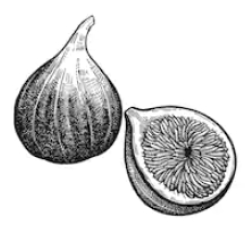
\includegraphics[width=1in,height=1.25in,clip,keepaspectratio]{fig1}}]{Michael Shell}
Use $\backslash${\tt{begin\{IEEEbiography\}}} and then for the 1st argument use $\backslash${\tt{includegraphics}} to declare and link the author photo.
Use the author name as the 3rd argument followed by the biography text.
\end{IEEEbiography}

\vspace{11pt}

\bf{If you will not include a photo:}\vspace{-33pt}
\begin{IEEEbiographynophoto}{John Doe}
Use $\backslash${\tt{begin\{IEEEbiographynophoto\}}} and the author name as the argument followed by the biography text.
\end{IEEEbiographynophoto}




\vfill

\end{document}


